
\documentclass[11pt,a4paper]{article}
\input{tutorial_style}
\begin{document}
\tutorialtitle{Note 1: Cyber Control and Game Learning}{Sampled-Data Control, RL/DRL, MARL/MAPPO, and Evaluation}{Dynamics, action timing, MDPs, RL/DRL, MARL/MAPPO, and evaluation}{Prepared for advanced research discussion and supervision}
\tableofcontents
\newpage
\lhead{\small\sffamily Note 1: Cyber Control and Game Learning}
\section{How This Guide Is Organized}
The note is organized around a clean workflow:
\begin{equation}
\begin{array}{c}
\boxed{\text{cyber dynamics}}\rightarrow\boxed{\text{control/game objective}}\rightarrow\boxed{\text{continuous-time theory}}\\[0.4em]
\rightarrow\boxed{\text{learning formulation}}\rightarrow\boxed{\text{implementation and evaluation}}
\end{array}
\end{equation}
The most important improvement is that RL, DRL, and MARL are not presented as unrelated tools after PMP. Instead, the note explains exactly how a continuous-time optimal control or differential game is converted into an MDP or Markov game, and what information from PMP is preserved or lost in that conversion.

\begin{boxednote}
\textbf{Key methodological principle.}
PMP and differential games define the continuous-time mathematical problem. RL/DRL/MARL usually solve a discretized feedback-control problem derived from that problem. PINN/PIDL can either learn unknown dynamics, solve the PMP residual system, or approximate HJB/HJI equations. These are different levels of coupling, and they should not be confused.
\end{boxednote}



\section{Notation and Method Selection}
This note uses a small number of repeated symbols. The same notation is used across optimal control, differential games, RL, and PINN/PIDL so that the link among methods is visible.

\begin{longtable}{p{0.20\textwidth}p{0.70\textwidth}}
\toprule
Symbol & Meaning \\
\midrule
$x(t)$ & continuous-time cyber state, for example malware compartments, APT asset states, or misinformation populations \\
$u_D(t),u_A(t)$ & continuous-time defender and attacker controls \\
$a_D^k,a_A^k$ & discrete-time actions selected at decision epoch $t_k$ \\
$t_k$ & action/observation point in the sampled MDP or Markov game after conversion \\
$\Delta t_k=t_{k+1}-t_k$ & action interval; fixed $\Delta t$ is a special case, not a requirement \\
$\tau_j$ & impulse or event point already present in the original continuous-time or impulse model \\
$\theta$ & physical or propagation parameters, such as infection, repair, forgetting, deception-decay, or correction rates \\
$J_D,J_A$ & cumulative defender and attacker objectives in continuous time \\
$H$ & Hamiltonian used by PMP or differential-game optimality conditions \\
$\lambda(t)$ & costate or adjoint variable; it measures marginal value of changing the state \\
$s_k$ & RL/DRL/MARL state at decision epoch $t_k$; usually derived from $x(t_k)$ and observations \\
$r_k$ & reward over the interval $[t_k,t_{k+1}]$, usually negative running cost \\
$\policy$ & policy mapping states to actions, e.g., $\policy_D(a_D|s)$ \\
\bottomrule
\end{longtable}

\subsection{What each method consumes and outputs}
A useful way to avoid confusion is to ask what each method consumes as input and what it returns as output.
\begin{longtable}{p{0.18\textwidth}p{0.34\textwidth}p{0.34\textwidth}}
\toprule
Method & Main input & Main output \\
\midrule
PMP & ODE model, cost functional, constraints & optimality system: state, costate, stationarity, boundary conditions \\
FBSM & PMP optimality system and initial guess for controls & open-loop trajectory $u^*(t)$ and state $x^*(t)$ \\
RL/DQN & MDP simulator $(s,a,r,s')$ with discrete actions & feedback policy or Q-function $Q(s,a)$ \\
PPO/SAC/DDPG & simulator with continuous-valued or stochastic actions & feedback actor $\policy(a|s)$ and critic \\
MARL & Markov game simulator with multiple agents & attacker and defender policies, often with centralized critics \\
Neural ODE & observed trajectories and differentiable ODE solver & learned dynamics $\dot{x}=f_\theta(x,u,t)$ or residual term $g_\theta$ \\
PINN/PIDL & data, equations, constraints, priors, possibly PMP/HJI residuals & states, parameters, controls, costates, or value functions satisfying residual constraints \\
\bottomrule
\end{longtable}

\begin{boxednote}
\textbf{Practical selection rule.}
Use PMP/FBSM when the model is known, continuous, and low- to moderate-dimensional. Use RL/DRL when actions are operational decisions and feedback policies are needed. Use MARL when the attacker adapts. Use Neural ODE when the dynamics are partly unknown. Use PINN/PIDL when equations and constraints are important and data are sparse, or when one wants a neural solver for PMP/HJB/HJI residual systems.
\end{boxednote}


\section{Game Concepts Before Learning: What Exactly Is Being Solved?}\label{sec:game-concepts}
A source of confusion in recent learning-for-differential-games papers is that the word ``game'' may refer to several different mathematical objects. Before choosing PMP, FBSM, RL, DRL, MARL, MADRL, PINN, or PIDL, it is useful to identify the game type and the solution concept. Differential games extend optimal control from one decision maker to multiple strategic decision makers: each player controls the same evolving state, but each player evaluates the outcome through its own objective. This point is emphasized in classical dynamic-game theory \cite{isaacs1965,basar1999} and in cyber differential-game tutorials.

\subsection{A compact taxonomy for cyber differential games}
The following table is intended as a practical checklist for malware, APT, deception, and propaganda-war models.

\begin{longtable}{p{0.21\textwidth}p{0.33\textwidth}p{0.36\textwidth}}
\toprule
Dimension & Meaning & Typical cyber interpretation \\
\midrule
Zero-sum vs general-sum & In a zero-sum game, $J_A=-J_D$. In a general-sum game, each player has a different payoff. & Malware attacker-defender games may be approximated as zero-sum. Propaganda, compliance, and insider-assisted APT games are often general-sum because costs, reputational effects, and operational benefits are not exact negatives. \\
Deterministic vs stochastic & The state equation is an ODE or a stochastic process. & Most propagation models use deterministic ODEs for tractability. RL/MADRL can add stochasticity through random initial states, random attacks, noisy observations, or network sampling. \\
Nash vs Stackelberg & In Nash games, players decide simultaneously. In Stackelberg games, a leader commits first and a follower responds. & Attacker-defender malware control is often modeled as Nash. Security investment, auditing, and compliance guidance can be Stackelberg if the organization commits first and employees or attackers respond. \\
Open-loop vs feedback & Open-loop controls are functions of time. Feedback controls are functions of the observed state. & PMP/FBSM usually returns $u_i(t)$ for a fixed initial state. RL/MADRL usually returns $\pi_i(a_i|s)$ that adapts to the current state. \\
Flow, impulse, and continuous--impulsive hybrid & Flow controls act through $\dot{x}=f(\cdot)$. Impulses create jumps $x(\tau^+)=G(x(\tau^-),v)$. Continuous--impulsive hybrid models combine flow controls and reset maps. & Propaganda spending, patching, or monitoring affect transition rates. Human incident response, media-literacy campaigns, isolation, and takedown actions may be better modeled as impulses. \\
\bottomrule
\end{longtable}

\begin{boxednote}
\textbf{Why this taxonomy matters for learning.}
DQN, PPO, SAC, MADDPG, MAPPO, and other MADRL methods do not directly require the original PMP equations. They require an environment. The game taxonomy determines what the environment should contain: one agent or multiple agents; zero-sum or general-sum rewards; simultaneous or sequential actions; discrete modes, continuous-valued actions, or parameterized actions; flow-only transitions or impulse jumps.
\end{boxednote}

\subsection{Nash equilibrium in continuous time and in Markov games}
For a two-player continuous-time differential game,
\begin{equation}
\dot{x}(t)=f(x(t),u_1(t),u_2(t),t),\quad x(0)=x_0,
\end{equation}
with objectives $J_1(u_1,u_2)$ and $J_2(u_1,u_2)$, an open-loop Nash equilibrium $(u_1^*,u_2^*)$ satisfies
\begin{equation}
J_1(u_1^*,u_2^*)\ge J_1(u_1,u_2^*)\quad \text{for all }u_1,
\end{equation}
\begin{equation}
J_2(u_1^*,u_2^*)\ge J_2(u_1^*,u_2)\quad \text{for all }u_2,
\end{equation}
when the convention is payoff maximization. If the problem is written as cost minimization, the inequality directions are reversed. PMP gives necessary conditions for such equilibria by introducing one Hamiltonian and one costate system for each player. In nonzero-sum games these conditions are normally necessary rather than sufficient, so numerical comparison against alternative strategies remains important.

After time discretization, state observation, action selection, and ODE/impulse simulation, the same strategic idea becomes a Markov game:
\begin{equation}
\mathcal{G}=\big(\mathcal{N},\mathcal{S},\{\mathcal{A}_i\}_{i\in\mathcal{N}},P,\{r_i\}_{i\in\mathcal{N}},\gamma\big).
\end{equation}
Here $\mathcal{N}$ is the player set, $\mathcal{S}$ is the state space, $\mathcal{A}_i$ is player $i$'s action space, $P(s'|s,a_1,\ldots,a_N)$ is the transition kernel, $r_i$ is the reward of player $i$, and $\gamma$ is a discount factor. A Markov-perfect Nash equilibrium is a profile of feedback policies $\pi_i^*(a_i|s)$ such that no player can improve its value by unilateral deviation:
\begin{equation}
V_i^{\pi_i^*,\pi_{-i}^*}(s)\ge V_i^{\pi_i,\pi_{-i}^*}(s),\quad \forall \pi_i,\; \forall s.
\end{equation}
This is the precise object that MARL and MADRL try to approximate.

\subsection{How the HODGE propaganda-war paper fits this taxonomy}
The HODGE/ORIENTATION framework is a useful example because it is not a simple continuous-control game. It combines a degree-based network model for dual competitive information spreading with a continuous--impulsive mechanism: continuous-time propaganda investment and discrete-time impulsive counter-propaganda investment \cite{cheng2024propaganda}. In words, propaganda is modeled as persistent influence over an interval, while counter-propaganda is modeled as targeted interventions at selected moments. This distinction is exactly the distinction between continuous flow control and impulse/jump control.

A simplified abstraction is
\begin{equation}
\dot{x}(t)=f(x(t),u_R(t),u_B(t)),\quad t\notin \tau_R\cup\tau_B,
\end{equation}
\begin{equation}
x(\tau_i^+)=G_R(x(\tau_i^-),v_R(\tau_i))\quad \text{or}\quad
x(\tau_i^+)=G_B(x(\tau_i^-),v_B(\tau_i)),
\end{equation}
where $u_R,u_B$ are continuous propaganda investment rates and $v_R,v_B$ are impulsive counter-propaganda investment levels. The original HODGE algorithm approximates a Nash strategy profile by iteratively updating continuous and impulsive decisions. A learning-based extension would not simply ``replace PMP by MADRL.'' Instead, it would define a Markov game in which each party observes a state summary, selects continuous and/or impulsive investment actions at decision epochs, applies jump maps if an impulse is selected, integrates the degree-based ODE until the next decision epoch, and receives a reward based on narrative benefit minus investment cost.

\begin{flowbox}
\textbf{Continuous--impulsive propaganda game as a Markov game}\par
Observe degree-based state summary $s_k$\par
$\Downarrow$\par
Red chooses $(m_R^k,v_R^k,u_R^k)$, Blue chooses $(m_B^k,v_B^k,u_B^k)$\par
$\Downarrow$\par
If $m_i^k$ is impulsive, apply jump map $G_i$\par
$\Downarrow$\par
Integrate ODE with continuous investments over $[t_k,t_{k+1}]$\par
$\Downarrow$\par
Compute rewards: influence benefit $-$ continuous cost $-$ impulse cost\par
$\Downarrow$\par
Update MADRL policies by self-play or CTDE
\end{flowbox}


\section{Cyber Dynamic Models: What Is Being Controlled?}
\subsection{Controlled malware propagation}
A basic malware or virus propagation model is
\begin{align}
    \dot{S}(t)&=-\beta S(t)I(t)-u_p(t)S(t)+\omega R(t), \\
    \dot{I}(t)&=\beta S(t)I(t)-\gamma I(t)-u_c(t)I(t), \\
    \dot{R}(t)&=\gamma I(t)+u_p(t)S(t)+u_c(t)I(t)-\omega R(t).
\end{align}
Here $S(t)$ denotes vulnerable devices, $I(t)$ compromised devices, and $R(t)$ recovered or protected devices. The infection term $\beta SI$ expresses the idea that vulnerable devices are compromised through interaction with infected devices. The control $u_p(t)$ represents patching or hardening, and $u_c(t)$ represents cleaning, monitoring, or incident response.

This model is suitable for introducing optimal control because the defender must balance two competing goals: reduce $I(t)$ and avoid excessive control cost. A typical objective is
\begin{equation}
J_D(u_p,u_c)=\int_0^T\left[A_I I(t)+\frac{B_p}{2}u_p^2(t)+\frac{B_c}{2}u_c^2(t)\right]\dd t+A_T I(T).
\end{equation}
The term $A_I I(t)$ is security loss, while $B_pu_p^2/2$ and $B_cu_c^2/2$ penalize aggressive intervention. The terminal term $A_T I(T)$ penalizes residual compromise.

\subsection{APT repair and deception dynamics}
APT attacks are persistent and stealthy, so it is useful to include repair, isolation, and deception. A compact APT-oriented model is
\begin{align}
    \dot{V} &= -\beta(1-\chi\eta_k)VC-u_hV+\omega P, \\
    \dot{C} &= \beta(1-\chi\eta_k)VC-(\gamma+u_r+u_i)C, \\
    \dot{P} &= u_hV+(\gamma+u_r+u_i)C-\omega P.
\end{align}
Here $V$ is vulnerable but uncompromised assets, $C$ is compromised assets, and $P$ is protected or repaired assets. The action $\eta_k\in[0,1]$ is chosen at decision epoch $t_k$ and held or mapped over the next interval. The factor $(1-\chi\eta_k)$ reduces the effective compromise rate during that interval. In cyber terms, honeypots, decoys, moving-target defense, or false information reduce useful attacker contact without introducing a fourth core compartment. This extends differential-game APT repair ideas such as Yang et al. \cite{yang2019apt} and connects naturally with impulsive and continuous--impulsive APT defense models \cite{sun2023impulsive,qin2024impulsive}.

\subsection{Rumor and misinformation defense}
For rumor, misinformation, or cyber propaganda, a simple correction model is
\begin{align}
    \dot{U} &= -\beta_MUM-\beta_CUC, \\
    \dot{M} &= \beta_MUM-\alpha MC-\delta M-u_fM, \\
    \dot{C} &= \beta_CUC+\alpha MC+u_fM-\delta_CC, \\
    \dot{R} &= \delta M+\delta_CC.
\end{align}
$U$ is unaware users, $M$ misinformation believers or spreaders, $C$ correction believers or counter-message spreaders, and $R$ inactive or removed users. The control $u_f(t)$ represents fact-checking, trusted correction, platform intervention, or public communication. This model makes sense for cyber propaganda games, where opposing sides can strategically influence narrative populations \cite{cheng2024propaganda}.

\begin{boxednote}
\textbf{Common structure.}
Malware, APT, and misinformation models all have the form
\[
\dot{x}=f(x,u_D,u_A,\theta,t),
\]
where $x$ is a cyber/social state, $u_D$ is defense intervention, $u_A$ is attack effort, and $\theta$ contains propagation parameters. This common structure is why PMP, FBSM, HJB/HJI, RL/DRL/MARL, Neural ODE, and PINN/PIDL can be studied in one framework.
\end{boxednote}



\subsection{How to read these models operationally}
The compartment variables should not be interpreted as only biological analogies. In cybersecurity, a compartment can represent a proportion of devices, accounts, hosts, services, narratives, or users. For example, $I(t)$ in a malware model can be the fraction of compromised IoT devices, while $M(t)$ in a misinformation model can be the fraction of users currently spreading a false narrative. A control is any costly intervention that changes transition rates. Patching changes the transition from vulnerable to protected. Cleaning changes the transition from compromised to recovered. Fact-checking changes the transition from misinformation to correction. Deception changes the effective attack rate by altering the attacker's information.

The main modeling decision is therefore not the name of the compartments but the transition mechanism. A paper should explain why each term exists. For example, $\beta SI$ means mass-action infection: compromise increases when both vulnerable and infected assets are present. The term $(1-\chi\eta_k)$ means a deception action reduces useful attacker contact over a decision interval. The term $u_fM$ means correction effort converts misinformation spreaders into corrected or inactive users. Clear interpretation of every term is essential before applying PMP or learning methods.

\subsection{What makes a cyber model suitable for learning-based control?}
A model is suitable when it can be simulated under candidate actions. For RL/DRL/MARL, the simulator may be an ODE solver, an agent-based simulator, a cyber range, or a sampled-data environment with optional impulse resets. For PINN/PIDL, the model must provide differentiable residuals or differentiable approximations. For Neural ODE, one needs trajectory data or simulated traces to train the dynamics. For PMP/FBSM, the model should be differentiable with respect to states and controls so that $H_x$, $H_u$, and costate equations can be derived.


\section{Control Timing, Action Spaces, and State Effects}\label{sec:continuous-discrete-impulse}

Cyber-control papers often use the words \emph{continuous}, \emph{discrete}, \emph{impulsive}, and \emph{hybrid} without naming the axis. A clean model states three independent choices:
\begin{enumerate}
\item \textbf{Decision timing:} is the decision a signal over time, a sampled decision at $t_k$, or an event decision at $\tau_j$?
\item \textbf{Action-value domain:} is the value real-valued, a discrete mode, or a parameterized pair $(m_k,v_k)$?
\item \textbf{State effect:} does the action change only the vector field, create a reset $x^+=G(x^-,v)$, or do both?
\end{enumerate}

\begin{figure}[htbp]
\centering
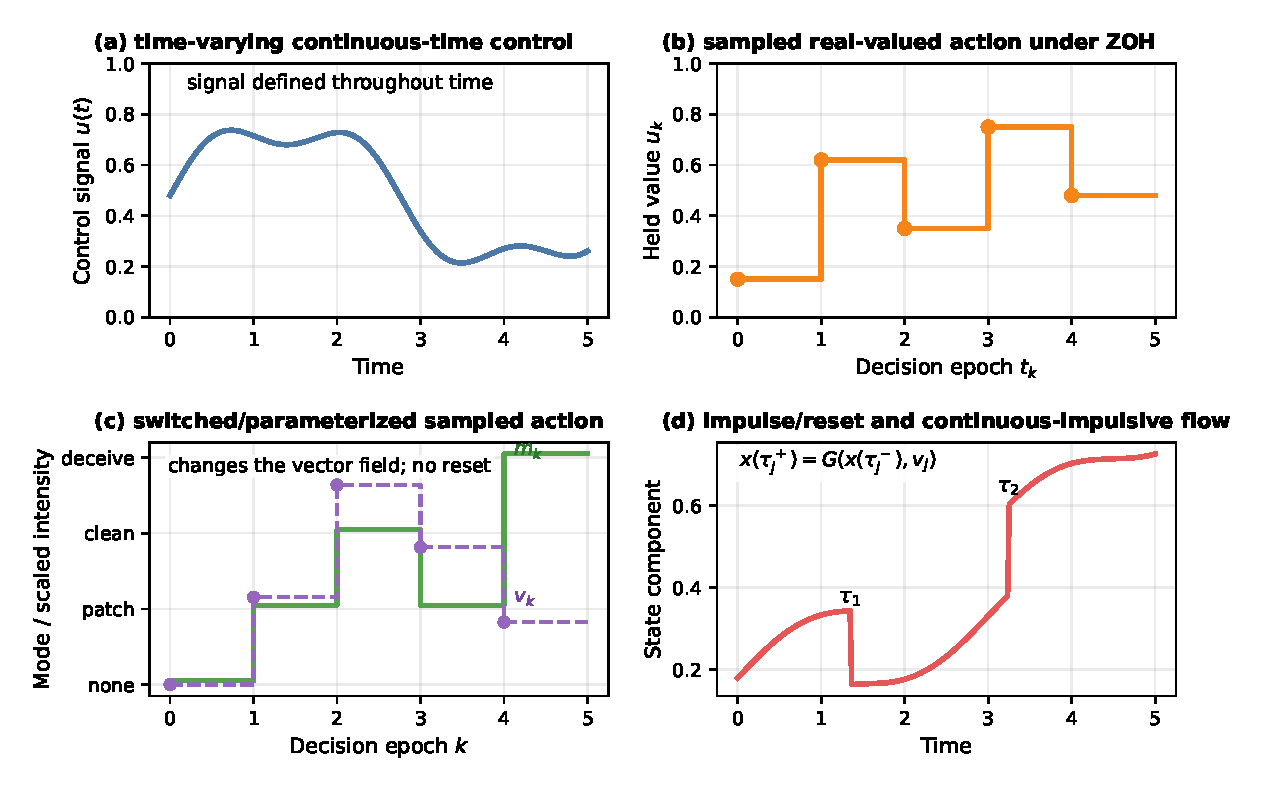
\includegraphics[width=0.95\linewidth]{../assets/control_action_taxonomy.pdf}
\caption{Control-action taxonomy used in this note. A continuous-time control is a time signal $u(t)$. A sampled real action $u_k$ under zero-order hold is piecewise constant. A mode or parameterized action selects the interval vector field without a reset unless a jump map is specified. An impulse is defined by the reset $x(\tau_j^+)=G(x(\tau_j^-),v_j)$.}
\label{fig:control-action-taxonomy}
\end{figure}

\subsection{Classification axes}
The same cyber intervention can look different depending on the axis. For example, a patching intensity $u_k=0.7$ chosen every hour is continuous-valued, but its decision timing is sampled and its applied signal is piecewise constant under zero-order hold. A mode $\texttt{patch}$ is discrete-valued, but the state can still evolve continuously with no jump. Isolation becomes impulsive only if it immediately changes the state.

\begin{boxednote}
\textbf{Common terminology errors.}
Use \emph{continuous-valued sampled action} for a real action chosen at $t_k$. Use \emph{continuous--impulsive hybrid control} only when the model states both the flow and reset semantics. A sampled mode switch with $x(t_k^+)=x(t_k^-)$ is switched or mode control, not an impulse.
\end{boxednote}

\subsection{Time-varying continuous-time control}
A continuous-time control signal is defined throughout the horizon:
\begin{equation}
    \dot{x}(t)=f(x(t),u(t),t),\qquad u(t)\in U,\quad t\in[0,T].
\end{equation}
The signal may vary inside any interval. Theory usually assumes measurable or piecewise-continuous controls, not that $u(t)$ must be smooth. It may be open-loop, $u(t)$, or feedback, $u(t)=\pi(x(t),t)$.

For a malware model,
\begin{equation}
\dot{S}=-\beta SI-u_p(t)S,\qquad
\dot{I}=\beta SI-(\gamma+u_c(t))I,
\end{equation}
where $u_p(t)$ and $u_c(t)$ are time-varying flow controls. PMP and FBSM solve for trajectories of this form. Detailed derivations remain in the foundation repository; Note 1 uses these controls mainly as baselines for learning experiments.

\subsection{Sampled-data control and zero-order hold}
Most RL environments choose actions at decision epochs
\begin{equation}
    0=t_0<t_1<\cdots<t_K=T,\qquad \Delta t_k=t_{k+1}-t_k.
\end{equation}
At $t_k$, the policy chooses $a_k$. Under zero-order hold,
\begin{equation}
    u(t)=\Gamma(a_k),\qquad t\in[t_k,t_{k+1}),
\end{equation}
with no reset:
\begin{equation}
    x(t_k^+)=x(t_k^-).
\end{equation}
If $a_k=u_k\in\mathbb{R}^m$, the action value is continuous-valued, but the applied signal is still piecewise constant. This is the bridge used by DQN/DDQN, PPO, SAC, and many Markov-game simulators.

\begin{flowbox}
Sampled-data ZOH transition:\\[0.3em]
observe $x(t_k)$ $\rightarrow$ choose $a_k$ $\rightarrow$ hold $\Gamma(a_k)$ on $[t_k,t_{k+1})$ $\rightarrow$ integrate ODE $\rightarrow$ return $x(t_{k+1})$.
\end{flowbox}

\subsection{Switched modes and parameterized actions without jumps}
A discrete mode can select a vector field:
\begin{equation}
    m_k\in\{1,\ldots,M\},\qquad
    \dot{x}=f_{m_k}(x,t),\quad t\in[t_k,t_{k+1}).
\end{equation}
If the action is $a_k=(m_k,v_k)$ with $v_k\in V_{m_k}$, call it a parameterized or mixed action:
\begin{equation}
    \dot{x}=f_{m_k}(x,v_k,t),\qquad x(t_k^+)=x(t_k^-).
\end{equation}
The mode and intensity define the action space. They do not by themselves define hybrid dynamics. In learning code this distinction matters: a mode/intensity actor changes rates over the interval, while the replay transition remains a flow-only sampled-data transition unless a jump map is called.

\subsection{Impulse and reset control}
An impulse is defined by an instantaneous state reset:
\begin{equation}
\begin{cases}
\dot{x}(t)=f(x(t),u(t),t), & t\neq \tau_j,\\[0.2em]
x(\tau_j^+)=G(x(\tau_j^-),v_j), & t=\tau_j.
\end{cases}
\end{equation}
The event time is $\tau_j$, not necessarily a learning epoch $t_k$. In cybersecurity, isolation, forced password reset, takedown, emergency cleanup, or mass warning can be modeled this way if they immediately move mass between compartments or remove nodes from an active set.

For SIR malware defense, a simple reset is
\begin{equation}
\begin{bmatrix}S(\tau_j^+)\\ I(\tau_j^+)\\ R(\tau_j^+)\end{bmatrix}
=
\begin{bmatrix}
(1-p_j)S(\tau_j^-)\\
(1-q_j)I(\tau_j^-)\\
R(\tau_j^-)+p_jS(\tau_j^-)+q_jI(\tau_j^-)
\end{bmatrix}.
\end{equation}
The reward or payoff must keep running and jump costs separate:
\begin{equation}
    r_k=-\int_{t_k}^{t_{k+1}}L(x(t),a_k)\,\dd t-C_{\rm imp}(x(t_k^-),v_k).
\end{equation}

\subsection{Continuous--impulsive hybrid control and games}
In this note, \emph{continuous--impulsive hybrid control} means flow control plus impulse resets:
\begin{align}
\dot{x}(t)&=f(x(t),u(t),m(t),t),\qquad t\neq \tau_j,\\
x(\tau_j^+)&=G(x(\tau_j^-),v_j).
\end{align}
The flow control may be a true time-varying signal or a sampled/ZOH implementation. Discrete modes may also be present, but they should be named explicitly, for example switched continuous--impulsive control.

For an attacker--defender game,
\begin{align}
\dot{x}&=f(x,u_A(t),u_D(t),m_A,m_D,t),\qquad t\neq \tau_j,\\
x(\tau_j^+)&=G(x(\tau_j^-),v_{A,j},v_{D,j}).
\end{align}
A sampled Markov game with $a_i^k=(m_i^k,v_i^k)$ and no reset is a parameterized-action Markov game. It becomes continuous--impulsive only when the simulator applies a reset. Broader hybrid-systems literature sometimes includes switched modes under the hybrid umbrella; this repository uses explicit labels so code and captions remain unambiguous.

\subsection{Method mapping}
\begin{longtable}{p{0.25\textwidth}p{0.32\textwidth}p{0.33\textwidth}}
\toprule
Model object & Mathematical form & Suitable method \\
\midrule
Time-varying flow control & $\dot{x}=f(x,u(t),t)$ & PMP, FBSM, direct collocation, MPC; foundation details \\
Sampled discrete action & $u(t)=\Gamma(a_k)$, $a_k\in\mathcal A$ & DQN/DDQN, tabular RL, action masks \\
Sampled continuous-valued action & $u(t)=u_k$ on $[t_k,t_{k+1})$ & PPO, SAC, DDPG, MPC-style actors \\
Switched or parameterized action & $a_k=(m_k,v_k)$, no reset & Parameterized-action RL, mixed-action policies, CTDE critics \\
Impulse/reset & $x^+=G(x^-,v)$ & Impulse control, semi-MDPs, event-triggered RL \\
Continuous--impulsive game & flow controls plus reset maps & Continuous--impulsive game conditions or a Markov-game simulator with explicit flow and reset costs \\
\bottomrule
\end{longtable}


\section{From Continuous-Time Control to MDPs and Markov Games}
This section is the bridge that is often missing in papers. It explains how a continuous-time optimal control or differential game becomes a discrete-time learning environment.

\subsection{Original continuous-time optimal control problem}
A defender-only control problem is
\begin{align}
\min_{u_D(\cdot)} \quad &J_D=\Phi(x(T))+\int_0^T L_D(x(t),u_D(t),t)\dd t, \\
\text{s.t.}\quad &\dot{x}(t)=f(x(t),u_D(t),t),\qquad x(0)=x_0.
\end{align}
PMP and FBSM solve this problem directly in continuous time. RL and DRL usually solve a derived discrete-time feedback-control problem.

\subsection{Does learning always require discretization?}
No. There are several different meanings of ``discretization,'' and confusing them leads to unclear papers.

\begin{longtable}{p{0.24\textwidth}p{0.36\textwidth}p{0.30\textwidth}}
\toprule
Object & What is discretized & Is it required? \\
\midrule
Continuous-time PMP/FBSM & A numerical mesh is used to solve ODE and costate equations. & Required for computation, but it is not an MDP. \\
Model-free RL or MARL & The learner receives transitions at action points $t_k$. & Usually required because replay buffers and Bellman updates use $(s_k,a_k,r_k,s_{k+1})$. \\
PINN, PIDL, Neural ODE & Collocation points or observed times are sampled. & Required for training data or residuals, but the learned object may still represent continuous time. \\
\bottomrule
\end{longtable}

Therefore, learning-based methods do not always require turning the original model into a simple discrete-time MDP. Model-free DQN, PPO, SAC, and MADRL usually do. PINN/PIDL and Neural ODE can keep a continuous-time residual and train on sampled points. FBSM uses a mesh for numerical integration but still solves the continuous-time optimality system.

\begin{boxednote}
\textbf{Piecewise constant is common, not mandatory.}
When an RL action is chosen at $t_k$, the simplest implementation is zero-order hold:
\[
u(t)=\Gamma(a_k),\qquad t\in[t_k,t_{k+1}).
\]
This makes the applied control piecewise constant on each action interval. It is common because it gives a clean environment transition. It is not required by the original differential game. One may use piecewise-linear controls, event-triggered impulses, continuous actor outputs inside a differentiable ODE solver, or a feedback law $u(t)=\pi(x(t),t)$ evaluated continuously. If a paper uses zero-order hold, it should say so explicitly.
\end{boxednote}

\subsection{Decision epochs, impulse times, and nonuniform intervals}
Use separate symbols for two different kinds of time points:
\[
0=t_0<t_1<\cdots<t_K=T,\qquad \Delta t_k=t_{k+1}-t_k,
\]
where $t_k$ is a learning action/observation point after conversion to an MDP or Markov game. The intervals $\Delta t_k$ do \emph{not} need to be equal. A fixed grid $t_k=k\Delta t$ is only the simplest implementation.

If the original continuous-time or impulse model already has event points, denote them by $\tau_j$. These points belong to the original model, not automatically to the RL conversion.

\begin{figure}[htbp]
\centering
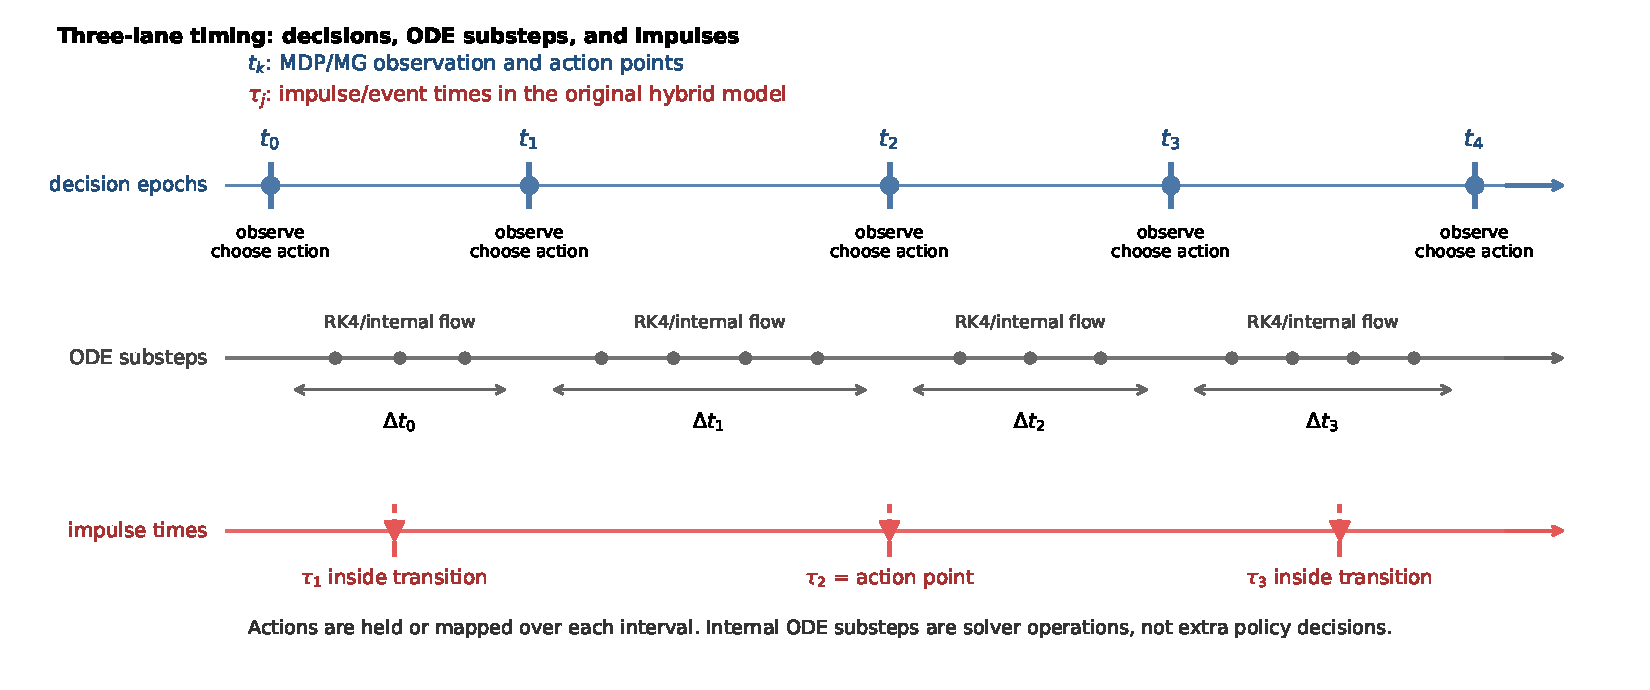
\includegraphics[width=0.95\linewidth]{../assets/action_timing.pdf}
\caption{Three-lane action timing used in the sampled-data learning code. Decision epochs $t_k$ are the points where the MDP or Markov game observes the state and chooses actions. ODE substeps are internal numerical integration steps. Impulse times $\tau_j$ belong to the original continuous-time or impulse model and may coincide with, or fall between, decision epochs.}
\label{fig:action-timing}
\end{figure}

\begin{longtable}{p{0.22\textwidth}p{0.36\textwidth}p{0.32\textwidth}}
\toprule
Relationship & Meaning & Implementation choice \\
\midrule
$\tau_j=t_k$ for selected $j,k$ & An original impulse event coincides with a learning action point. & Expose the impulse as an available action or mode at that epoch. \\
$\{\tau_j\}\subset\{t_k\}$ & Only some decision epochs allow emergency actions. & Add an action mask or time-dependent action set. \\
$\tau_j\in(t_k,t_{k+1})$ & The original model has an event inside a learning transition. & Apply the event inside the simulator transition and include its effect in $s_{k+1}$ and $r_k$. \\
$\tau_j$ chosen by policy & The action includes event timing. & Use a semi-MDP, event-triggered policy, or waiting-time action. \\
\bottomrule
\end{longtable}

In this repository, the default code convention is simple: the policy observes $x(t_k^-)$, chooses an action, the environment applies any jump to obtain $x(t_k^+)$, then it integrates the ODE to the next observation $x(t_{k+1}^-)$. This is the convention used in \texttt{sampled\_continuous\_impulse\_env.py}. The code uses fixed \texttt{EnvConfig.dt}; the mathematics above allows nonuniform action schedules.

\subsection{Step-by-step conversion to an MDP}
At each $t_k$, the defender observes the pre-jump state summary
\begin{equation}
s_k=\psi(x(t_k^-),b_k,o_k),
\end{equation}
where $b_k$ may represent budget and $o_k$ may represent observations such as alerts or detection scores. The defender chooses an action $a_k$. The action can be a discrete mode, a continuous-valued vector, or a parameterized pair:
\begin{align}
\text{discrete: }&a_k\in\{\text{patch},\text{monitor},\text{isolate},\text{deceive}\},\\
\text{continuous: }&a_k=[u_p^k,u_c^k,u_d^k]\in[0,1]^3,\\
\text{parameterized: }&a_k=(m_k,v_k),\quad m_k\in\{\text{patch},\text{monitor},\text{deceive}\},\; v_k\in[0,1].
\end{align}
If $a_k$ has an impulse component, the environment first applies a jump map
\begin{equation}
y_k=x(t_k^+)=G(x(t_k^-),a_k).
\end{equation}
If there is no impulse component, then $y_k=x(t_k^-)$. The continuous dynamics then run between decision points:
\begin{equation}
x_{k+1}^-=\ODESolve\left(f,y_k,a_k,[t_k,t_{k+1})\right).
\end{equation}
The reward is the negative of the interval cost:
\begin{equation}
r_k=-C_{\rm jump}(x(t_k^-),a_k)-\int_{t_k}^{t_{k+1}}L_D(x(t),a_k,t)\dd t.
\end{equation}
A simple numerical approximation is
\begin{equation}
r_k\approx -C_{\rm jump}(x(t_k^-),a_k)-\Delta t_k\,L_D(x_{k+1}^-,a_k,t_{k+1}).
\end{equation}
Now the problem is an MDP
\begin{equation}
(\mathcal{S},\mathcal{A},P,r,\gamma_k),
\end{equation}
where $P$ is generated by the ODE solver, jump map, and stochastic disturbances. This is the correct Level 1 bridge from optimal control to RL \cite{sutton2018}.

\begin{flowbox}
\textbf{Continuous-time or impulse model to MDP}\\[0.3em]
$\dot{x}=f(x,u,t)$ and optional original impulses at $\tau_j$\quad
$\Longrightarrow$ choose action points $t_k$\quad
$\Longrightarrow$ observe $s_k=\psi(x(t_k^-))$\quad
$\Longrightarrow$ apply jumps/events, integrate flow, return $s_{k+1}$\quad
$\Longrightarrow$ reward $r_k\approx-C_{\rm jump}-\int L\dd t$\quad
$\Longrightarrow$ train RL/DRL policy $\pi(a|s)$.
\end{flowbox}

\subsection{Discounting and continuous-time costs}
If the original continuous-time objective uses discounting
\begin{equation}
J=\int_0^T e^{-\rho t}L(x(t),u(t))\dd t,
\end{equation}
then the interval-specific discrete discount can be chosen as
\begin{equation}
\gamma_k=e^{-\rho\Delta t_k}.
\end{equation}
For a fixed grid this becomes $\gamma_d=e^{-\rho\Delta t}$. If the original problem has a finite horizon and no discount, many implementations set $\gamma_d$ close to one and terminate at $K$. The key is to make the discrete reward consistent with the original running cost. Otherwise, the DRL policy may optimize a different problem from the one stated in the differential-game model.

\subsection{Action-to-control map}
A common source of confusion is the difference between a discrete RL action and a continuous control in the ODE. The bridge is an action-to-control map
\begin{equation}
\Gamma:\mathcal{A}\rightarrow\mathcal{U},\qquad u(t)=\Gamma(a_k),\quad t\in[t_k,t_{k+1}).
\end{equation}
For example,
\begin{equation}
\Gamma(\text{patch})=(u_p,u_c,u_d)=(0.8,0.1,0),
\end{equation}
while
\begin{equation}
\Gamma(\text{deceive})=(0.1,0.1,0.9).
\end{equation}
For a parameterized sampled action $a_k=(m_k,v_k)$, the map becomes
\begin{equation}
\Gamma(m_k,v_k)=v_k\Gamma_{max}(m_k),
\end{equation}
so the agent chooses both intervention type and intensity.

\subsection{A practical environment interface}
In code, the continuous-time model becomes an environment with two important functions:
\begin{methodbox}
\textbf{ODE-based cyber MDP interface.}
\begin{enumerate}
\item \texttt{reset}: sample or set $x_0$, budget $b_0$, attack scenario, and horizon $K$.
\item \texttt{observe}: return $s_k=\psi(x_k,o_k,b_k)$, where $o_k$ may be noisy alerts or partial measurements.
\item \texttt{step(a\_k)}: convert $a_k$ to ODE controls, integrate the dynamics for one interval, compute reward, update budget, and return $(s_{k+1},r_k,done)$.
\end{enumerate}
\end{methodbox}
The Markov property requires that $s_k$ contain enough information to predict the next state distribution given the action. If the defender observes only alerts rather than true compromise levels, the problem is closer to a partially observable MDP. A practical workaround is to include a history window, recurrent neural network, or state estimator.

\subsection{Conversion to a Markov game}
For an attacker-defender differential game,
\begin{align}
\dot{x}&=f(x,u_A,u_D,t),\\
J_D&=\Phi_D(x(T))+\int_0^T L_D(x,u_A,u_D,t)\dd t,\\
J_A&=\Phi_A(x(T))+\int_0^T L_A(x,u_A,u_D,t)\dd t.
\end{align}
Choose decision times. At step $k$, each player observes the state summary before any new jump:
\begin{equation}
a_A^k\sim\pi_A(\cdot|s_k),\qquad a_D^k\sim\pi_D(\cdot|s_k).
\end{equation}
The joint action may include impulse modes and continuous-flow modes. The transition is
\begin{equation}
x(t_k^+)=G(x(t_k^-),a_A^k,a_D^k),\qquad
s_{k+1}=\psi\!\left(\ODESolve(f,x(t_k^+),a_A^k,a_D^k,[t_k,t_{k+1}))\right),
\end{equation}
and rewards are
\begin{align}
r_D^k&\approx-\Delta t_k\,L_D(s_{k+1},a_A^k,a_D^k),\\
r_A^k&\approx\Delta t_k\,L_A(s_{k+1},a_A^k,a_D^k).
\end{align}
This gives a Markov game
\begin{equation}
(\mathcal{S},\mathcal{A}_A,\mathcal{A}_D,P,r_A,r_D,\gamma_d).
\end{equation}
MARL learns policies $\pi_A$ and $\pi_D$ by repeated interaction.

\subsection{What is preserved and what is lost?}
This conversion preserves the state dynamics, intervention costs, and strategic interaction. However, it usually does not preserve the costate equations or Hamiltonian stationarity conditions unless these are explicitly added to the learning objective. Therefore, a DRL solver for the induced MDP is not automatically a solver for the PMP boundary-value problem. It is a feedback-policy solver for a discretized control/game problem.

\section{PMP/FBSM Baseline Bridge}
\begin{boxednote}
\textbf{Scope of this section.}
This note uses PMP and FBSM only as a short bridge from continuous-time models to learning baselines. The detailed optimal-control derivations, FBSM implementation choices, and classical differential-game examples are maintained in the Foundation repository.
\end{boxednote}

For a known continuous-time model
\[
\dot{x}=f(x,u,t),\qquad J=\Phi(x(T))+\int_0^T L(x,u,t)\dd t,
\]
PMP introduces a Hamiltonian
\[
H(x,u,\lambda,t)=L(x,u,t)+\lambda^\top f(x,u,t),
\]
and gives state, costate, stationarity, and terminal conditions \cite{pontryagin1962,lenhart2007}. FBSM solves the resulting two-point boundary-value problem iteratively:
\begin{flowbox}
Guess $u^{(0)}(t)$ $\rightarrow$ forward solve $x^{(i)}(t)$ $\rightarrow$ backward solve $\lambda^{(i)}(t)$ $\rightarrow$ update $u^{(i+1)}(t)$ $\rightarrow$ repeat.
\end{flowbox}

\subsection{FBSM versus RL/DRL: what changes?}
FBSM normally returns an open-loop control $u^*(t)$ for a fixed initial condition and fixed parameters. If the cyber state deviates from the predicted trajectory, the schedule may be suboptimal unless the problem is solved again. RL/DRL instead learns a feedback policy $\policy(a|s)$ that reacts to the observed state.

\begin{longtable}{p{0.22\textwidth}p{0.34\textwidth}p{0.34\textwidth}}
\toprule
Aspect & FBSM/PMP & RL/DRL/MARL \\
\midrule
Control type & time-varying signal & discrete mode, continuous-valued, or parameterized sampled action \\
Output & open-loop trajectory $u(t)$ & feedback policy $\policy(a|s)$ \\
Theory & strong optimality interpretation under assumptions & approximate, data/simulation-driven \\
Need derivatives & yes, $H_x,H_u$ & no analytic derivatives needed \\
Adaptation & requires re-solving or feedback extension & policy directly reacts to state \\
Discrete modes & awkward unless switching/impulse control is used & natural \\
Training cost & usually cheap for low-dimensional ODEs & can be expensive due to many episodes \\
Interpretability & high & medium to low, unless policy is analyzed \\
\bottomrule
\end{longtable}

A useful experimental design is to treat FBSM as a continuous-control benchmark and DRL as a feedback controller. If DRL is claimed to improve FBSM, explain whether the improvement comes from feedback adaptation, discrete action modeling, robustness to stochasticity, or optimizing a different objective.

\subsection{How PMP should be connected to learning}
\begin{longtable}{p{0.11\textwidth}p{0.24\textwidth}p{0.53\textwidth}}
\toprule
Level & Name & Meaning \\
\midrule
0 & Disconnected learning & PMP is derived, but RL/DRL ignores $H$, $\lambda$, and $H_u$. It only uses simulator rewards. \\
1 & PMP-formulated RL/DRL & PMP/differential-game theory defines the continuous-time model and payoff; RL solves the induced MDP or Markov game. This is common in DDQN malware and PPO deception studies \cite{shen2023ddqn,he2026timedelay,he2024deception}. \\
2 & PMP-assisted learning & FBSM/PMP controls are used as expert demonstrations, warm starts, reward shaping, or baselines. \\
3 & PMP-informed PINN/PIDL & The neural loss explicitly contains state residuals, costate residuals, stationarity residuals $\|H_u\|^2$, and boundary residuals. \\
4 & HJI/Pontryagin operator learning & The learner approximates value gradients or costate operators across states and parameters, as in Pontryagin neural operator work \cite{zhang2024pno}. \\
\bottomrule
\end{longtable}

\begin{boxednote}
\textbf{Writing advice.}
If a method trains on $(s,a,r,s')$ only, call it a DRL solver for the induced MDP or Markov game. If the loss contains $\dot{\lambda}+H_x$, $H_u$, or HJI residuals, call it PMP-informed or HJI-informed. This avoids overstating the connection between PMP and learning.
\end{boxednote}

PMP/FBSM gives structure but may be too slow, too offline, or too continuous for operational cyber actions. For example, DDQN malware suppression formulates the malware game and then uses DDQN because actions such as patching decisions are discrete \cite{shen2023ddqn}. Time-delay deception deployment formulates a differential game but converts it to a Markov game and uses PPO to learn real-time feedback policies \cite{he2026timedelay}. These are valid designs, but the methodological contribution is not ``solving PMP by DRL.'' It is ``using DRL to solve the feedback decision problem induced by a differential game.''

\section{RL and DRL in Cyber Control}
This section keeps the main ideas concise. Appendix \ref{app:rl-background} gives the prerequisite details.

\subsection{Why use RL?}
RL is useful when the defender can simulate the cyber system but cannot easily solve the analytic optimality system. It is also useful when actions are operational and discrete. In the MDP derived in Section 3, RL learns
\begin{equation}
\pi(a|s)\quad\text{or}\quad Q(s,a),
\end{equation}
so the defender can react to the current cyber state instead of following a precomputed open-loop control $u(t)$.

\subsection{DQN for discrete cyber actions}
For discrete actions such as no-op, patch, monitor, isolate, and deceive, DQN approximates $Q(s,a)$ using a neural network \cite{mnih2015}. The Bellman target is
\begin{equation}
y=r+\gamma_d\max_{a'}Q_{\theta^-}(s',a'),
\end{equation}
and the training loss is
\begin{equation}
\mathcal{L}_{DQN}(\theta)=\E_{(s,a,r,s')\sim\mathcal{D}}\left[\left(Q_\theta(s,a)-y\right)^2\right].
\end{equation}
Double DQN reduces overestimation by using the online network to select the next action and the target network to evaluate it \cite{vanhasselt2016ddqn}:
\begin{equation}
y^{DDQN}=r+\gamma_d Q_{\theta^-}\left(s',\argmax_{a'}Q_\theta(s',a')\right).
\end{equation}

\begin{methodbox}
\textbf{DQN implementation for malware defense.}
\begin{enumerate}
\item State: $s_k=[S_k,I_k,R_k]$, normalized to $[0,1]$; budget or context variables can be appended only when they are explicitly modeled.
\item Actions: $\{\text{no-op},\text{patch},\text{clean},\text{deceive},\text{isolate}\}$.
\item Transition: map the action to ODE parameters, integrate from $t_k$ to $t_{k+1}$.
\item Reward: $r_k=-\Delta t_k(A_II_{k+1}+c_a(a_k)+c_{iso}\mathbf{1}_{a_k=\text{isolate}}I_{k+1})$.
\item Network: MLP $3\to64\to64\to5$ for the default aggregate environment.
\item Training: replay buffer, target network, $\epsilon$-greedy exploration, Adam optimizer.
\end{enumerate}
\end{methodbox}

\subsection{Actor-critic methods for continuous controls}
If actions are continuous-valued intensities such as $u_p,u_c,u_d\in[0,1]$, DQN is inconvenient. Actor-critic methods learn a policy network and a value or Q network. DDPG learns a deterministic actor for continuous-valued actions \cite{lillicrap2015}; PPO uses a clipped policy-gradient objective for stable updates \cite{schulman2017}; SAC adds entropy regularization for exploration \cite{haarnoja2018}. A typical actor for cyber defense is
\begin{equation}
\pi_\theta(s)=\left[u_p(s),u_c(s),u_d(s)\right],\qquad u_i(s)=\sigmoid(h_i(s)).
\end{equation}



\subsection{DQN training loop in detail}
DQN learns from transitions rather than complete analytic equations. For an ODE-based malware environment, each transition is generated by solving the ODE for one decision interval. The training loop is:
\begin{enumerate}
\item Initialize the online Q-network $Q_\theta$ and target network $Q_{\theta^-}$.
\item At state $s_k$, choose a random action with probability $\epsilon$, otherwise choose $a_k=\argmax_aQ_\theta(s_k,a)$.
\item Run the ODE environment to obtain $(s_{k+1},r_k,done)$.
\item Store $(s_k,a_k,r_k,s_{k+1},done)$ in replay buffer $\mathcal{D}$.
\item Sample a mini-batch from $\mathcal{D}$ and compute Bellman targets.
\item Update $\theta$ by minimizing squared Bellman error.
\item Periodically copy $\theta$ to $\theta^-$ or use a soft update.
\end{enumerate}
Typical starting hyperparameters are replay buffer size $10^4$--$10^6$, mini-batch size 64--256, learning rate $10^{-4}$--$10^{-3}$, target update every 100--1000 gradient steps, and an $\epsilon$ schedule decreasing from 1 to 0.05. These values should be reported because they affect reproducibility.

\subsection{When to use DQN, PPO, SAC, or DDPG}
\begin{itemize}
\item Use \textbf{DQN/DDQN} when actions are a small set of discrete interventions such as patch, isolate, monitor, and deceive.
\item Use \textbf{PPO} when actions are discrete, continuous-valued, or parameterized and stable policy updates are more important than sample efficiency.
\item Use \textbf{DDPG/TD3/SAC} when controls are continuous resource intensities. SAC is often more robust because entropy encourages exploration.
\item Use \textbf{parameterized-action RL} when a decision has both a mode and a continuous intensity, for example patch at intensity 0.7.
\end{itemize}
A good paper should justify the algorithm from the action space and cyber decision structure, not just use a popular DRL method.

\subsection{Reward shaping without changing the problem too much}
Reward shaping is useful but dangerous. The base reward should be the negative running cost from the original optimal-control problem:
\begin{equation}
r_k^{base}\approx-\int_{t_k}^{t_{k+1}}L(x(t),a_k)\dd t.
\end{equation}
Additional terms can encourage containment or safe exploration, for example
\begin{equation}
r_k=r_k^{base}+\eta_1(C_k-C_{k+1})-\eta_2\ind\{C_{k+1}>C_{max}\}.
\end{equation}
However, if the shaping terms dominate, the DRL agent may solve a different problem. In research writing, list the base objective first and state clearly which shaping terms are added for training stability.

\section{MARL for Attacker-Defender Interaction}
\subsection{Markov game implementation}
A Markov game is used when the attacker adapts. At each step,
\begin{equation}
a_A^k\sim\pi_A(\cdot|s_k),\qquad a_D^k\sim\pi_D(\cdot|s_k),
\end{equation}
and the ODE environment returns $s_{k+1},r_A^k,r_D^k$. The defender and attacker update their policies using sampled trajectories.

\begin{flowbox}
\textbf{MARL interaction loop}\\[0.3em]
state $s_k$ $\rightarrow$ attacker action $a_A^k$ and defender action $a_D^k$ $\rightarrow$ ODE cyber transition $s_{k+1}$ $\rightarrow$ rewards $r_A^k,r_D^k$ $\rightarrow$ update $\pi_A,\pi_D$.
\end{flowbox}

\subsection{Concrete attacker-defender malware/deception game}
Use $s_k=[V_k,C_k,P_k]$. Defender actions are patch, monitor, isolate, deceive. Attacker actions are scan, exploit, lateral movement, stealth. Deception is modeled as an action effect over the current decision interval, not as a stored population compartment:
\[
\beta_k^{\rm eff}=\beta_k(1-\chi\eta_k).
\]
The ODE between decision points is
\begin{align}
\dot{V}&=-\beta_k^{\rm eff}VC-\rho_kV+\omega P,\\
\dot{C}&=\beta_k^{\rm eff}VC-(\gamma+\mu_k+\iota_k)C,\\
\dot{P}&=\rho_kV+(\gamma+\mu_k+\iota_k)C-\omega P.
\end{align}
The defender reward is
\begin{equation}
r_D^k=-\Delta t_k\left(w_CC_{k+1}+c_\rho\rho_k^2+c_\mu\mu_k^2+c_\iota\iota_k^2+c_\eta\eta_k^2+c_U\iota_kC_{k+1}\right),
\end{equation}
and the attacker reward is
\begin{equation}
r_A^k=\Delta t_k\left(q_CC_{k+1}-d_A(a_A^k)-q_PP_{k+1}\right).
\end{equation}

\subsection{Training order}
A stable training order is:
\begin{enumerate}
\item train defender against scripted attacker;
\item train attacker against fixed or pretrained defender;
\item start self-play from pretrained policies;
\item evaluate against unseen attackers and unseen defense costs.
\end{enumerate}
Independent learning is simple but unstable. Centralized training and decentralized execution (CTDE) improves stability by using critics such as
\begin{equation}
Q_D(s,a_A,a_D),\qquad Q_A(s,a_A,a_D),
\end{equation}
while actors execute using local observations. MADDPG and MAPPO are representative CTDE-style methods \cite{lowe2017,yu2021mappo}.



\subsection{Independent learning versus CTDE}
In independent learning, the attacker treats the defender as part of the environment and the defender treats the attacker as part of the environment. This is simple but can be unstable because each agent's learning changes the transition distribution for the other agent. CTDE addresses this by allowing the critic to see joint information during training:
\begin{equation}
Q_D(s,a_A,a_D),\qquad Q_A(s,a_A,a_D),
\end{equation}
while each actor still executes using its own observation. This is appropriate for cyber research because offline training may use complete simulator information, while deployment only uses observable alerts and measurements.

\subsection{Self-play curriculum for cyber games}
A practical MARL curriculum is:
\begin{enumerate}
\item train the defender against a weak scripted attacker;
\item train the defender against stronger scripted attackers;
\item freeze defender and train attacker to exploit it;
\item alternate attacker and defender updates;
\item evaluate against held-out attackers and randomized parameters.
\end{enumerate}
This curriculum is often more stable than starting from fully random self-play. It also produces interpretable experimental stages: basic containment, adaptive attack, and robust defense.


\subsection{MADRL algorithm families for attacker-defender games}
MARL is the broad field of reinforcement learning with multiple agents. MADRL is the deep-learning version, where policies, critics, or value functions are neural networks. For cyber differential games, four families are especially useful.

\begin{longtable}{p{0.22\textwidth}p{0.31\textwidth}p{0.37\textwidth}}
\toprule
Family & How it works & When it is suitable \\
\midrule
Independent DQN/PPO & Each agent treats the other agents as part of the environment and learns its own value or policy. & Simple baseline. Useful for small cyber games, but training can be unstable because the environment is nonstationary from each agent's view. \\
Self-play & Agents repeatedly train against recent or historical versions of opponents. & Good for attacker-defender cyber games where we want adaptive behavior rather than a policy overfitted to one fixed attacker. \\
Centralized critic, decentralized actors & During training, the critic sees joint actions and possibly global state; during execution, each actor uses local observation. & Useful for simultaneous attacker-defender decisions. MADDPG and MAPPO follow this spirit \cite{lowe2017,yu2021mappo}. \\
Opponent modeling / population training & Agents learn or sample from a population of opponent policies. & Useful when the defender must be robust against many attacker types, not just the latest self-play opponent. \\
\bottomrule
\end{longtable}

A common CTDE critic for player $i$ is
\begin{equation}
Q_i(s,a_1,\ldots,a_N;\phi_i),
\end{equation}
while the decentralized actor is
\begin{equation}
\pi_i(a_i|o_i;\theta_i),
\end{equation}
where $o_i$ may be a local observation rather than the full state. In an APT game, the defender may observe alerts and estimated compromise ratios, while the attacker may observe discovered vulnerable assets. The centralized critic is allowed to use the full simulator state during training because it is a training device, not an operational assumption.

\subsection{A step-by-step MADRL recipe for a cyber differential game}
For a two-player attacker-defender game, use the following sequence.
\begin{enumerate}
\item \textbf{Start from the continuous-time game.} Write $\dot{x}=f(x,u_A,u_D)$ and objectives $J_A,J_D$.
\item \textbf{Choose the action schedule.} Choose $0=t_0<t_1<\cdots<t_K=T$. A fixed interval $t_k=k\Delta t$ is convenient, but nonuniform intervals are also valid when operations are event-triggered or risk-triggered.
\item \textbf{Define observations.} Use $o_D^k=h_D(x(t_k))$ and $o_A^k=h_A(x(t_k))$. If both agents see the full state, the game is fully observed. If not, the practical model is a partially observed Markov game.
\item \textbf{Define actions.} Choose discrete modes, continuous-valued intensities, or parameterized actions. Example: defender action $a_D=(\text{deceive},0.7)$; attacker action $a_A=(\text{lateral movement},0.5)$.
\item \textbf{Apply impulse first if needed.} If the action is an incident-response impulse, compute $x(t_k^+)=G(x(t_k^-),a_A^k,a_D^k)$.
\item \textbf{Integrate the ODE.} Compute $x(t_{k+1})=\ODESolve(f,x(t_k^+),a_A^k,a_D^k,\Delta t_k)$.
\item \textbf{Compute rewards by interval integration.} For player $i$, set $r_i^k\approx \int_{t_k}^{t_{k+1}} L_i(x,u_A,u_D)\dd t$ plus any impulse reward/cost.
\item \textbf{Train policies.} Use independent PPO for a simple start, then MAPPO or MADDPG for CTDE.
\item \textbf{Evaluate game quality.} Report not only average reward but also best-response tests, exploitability proxies, robustness to unseen opponents, and comparison with PMP/FBSM or HODGE-style baselines.
\end{enumerate}

\subsection{Equilibrium evaluation in MADRL}
A trained pair of policies is not automatically a Nash equilibrium. In a paper, avoid saying that self-play ``finds the Nash equilibrium'' unless a meaningful equilibrium diagnostic is provided. Practical diagnostics include:
\begin{enumerate}
\item \textbf{Unilateral deviation test:} freeze the defender and retrain a new attacker best response. Then freeze the attacker and retrain a new defender best response.
\item \textbf{Exploitability proxy:} measure how much reward a best-response agent gains over the trained agent.
\item \textbf{Opponent pool robustness:} evaluate the defender against random, static, PMP/FBSM, HODGE-style, and learned attackers.
\item \textbf{Cost-effectiveness comparison:} compare cumulative security benefit minus control cost, similar in spirit to continuous--impulsive propaganda-war experiments \cite{cheng2024propaganda}.
\item \textbf{Structural sanity check:} verify that actions make cyber sense, e.g., early containment or deception when compromise grows, reduced spending when the system is already safe.
\end{enumerate}

\begin{boxednote}
\textbf{Important wording.}
For MADRL results, it is safer to write ``the learned policy profile is an approximate equilibrium candidate'' or ``a robust adaptive strategy profile'' unless best-response or exploitability analysis supports a stronger Nash claim.
\end{boxednote}

\subsection{How PMP/FBSM baselines strengthen MADRL papers}
A cyber MADRL paper is stronger when it is not compared only with random or static policies. PMP/FBSM or HODGE-style strategies can serve three roles.
\begin{enumerate}
\item \textbf{Baseline:} compare learned feedback policies with open-loop continuous-time strategies.
\item \textbf{Teacher:} generate state-action pairs from many initial states and pretrain the actor by behavior cloning.
\item \textbf{Validation:} evaluate whether learned actions approximately satisfy Hamiltonian stationarity in regions where the action space is continuous.
\end{enumerate}
For example, if PMP gives $u_D^{\mathrm{PMP}}(t)$ for an initial state $x_0$, simulate small perturbations of $x_0$, solve FBSM repeatedly, and train a policy $\pi_D(x,t)$ to imitate the resulting controls. Then fine-tune by RL/MADRL. This produces a more transparent bridge between differential-game theory and learning.

\section{Neural ODE and PINN/PIDL Handoff}
\begin{boxednote}
\textbf{Scope of this section.}
This note introduces Neural ODE, PINN, and PIDL only to explain how learning can be constrained by equations. Detailed inverse-learning, physics-informed, data-informed, and PMP-informed neural methods are maintained in Note 2.
\end{boxednote}

Neural ODE learns a continuous vector field, often written as
\[
\dot{x}=f_{\mathrm{known}}(x,u,t;\theta_p)+g_\theta(x,u,t),
\]
where the mechanistic part captures the cyber model and the neural term captures missing mechanisms such as attacker adaptation or unobserved platform effects \cite{chen2018neuralode}. It learns dynamics; it does not by itself choose an optimal action.

PINN/PIDL adds equation residuals, conservation laws, parameter priors, boundary conditions, and sometimes PMP/HJB/HJI residuals to the training loss \cite{raissi2019}. In this project family, Note 2 is the detailed reference for inverse SIR/SIPS learning, PIDL missing-mechanism models, direct neural control, and PMP-informed neural solvers. In Note 1, these methods are mainly used as upstream estimation tools or optional equation-informed baselines before RL/MARL evaluation.

\section{Parameterized Actions and Continuous--Impulsive Game Extensions}
\subsection{Why parameterized actions are useful}
In practice, a defender often chooses both a mode and an intensity:
\begin{equation}
a_D^k=(m_D^k,v_D^k),\quad m_D^k\in\{\text{patch},\text{monitor},\text{isolate},\text{deceive}\},\quad v_D^k\in[0,1].
\end{equation}
The attacker may choose
\begin{equation}
a_A^k=(m_A^k,v_A^k),\quad m_A^k\in\{\text{scan},\text{exploit},\text{lateral},\text{stealth}\},\quad v_A^k\in[0,1].
\end{equation}
Between decision times, these actions can select a flow field:
\begin{equation}
\dot{x}=f_{m_A^k,m_D^k}(x,v_A^k,v_D^k,t),\qquad t\in[t_k,t_{k+1}).
\end{equation}
If there is no reset, this is a parameterized-action sampled Markov game. It should not be called continuous--impulsive merely because the action has both a discrete and a real-valued component.

\subsection{Solution routes}
\paragraph{Route 1: mode enumeration plus PMP.}
Fix a mode sequence, solve continuous intensities by PMP/FBSM, and compare candidate sequences. This is interpretable but grows exponentially with the number of switching times.

\paragraph{Route 2: parameterized action RL.}
Use two policy heads \cite{hausknecht2015}:
\begin{equation}
\pi(s)=\left(\pi_m(m|s),\pi_v(v|s,m)\right).
\end{equation}
The first head selects a mode; the second outputs the intensity for that mode.

\paragraph{Route 3: parameterized-action MARL.}
Both attacker and defender use parameterized policies, and a centralized critic evaluates
\begin{equation}
Q(s,m_A,v_A,m_D,v_D).
\end{equation}
This is appropriate for sampled cyber games with discrete modes and real-valued intensities.

\paragraph{Route 4: relaxed PINN/PIDL.}
Represent discrete modes with soft weights
\begin{equation}
\omega_m(t)=\softmax(g_\theta(t)),\qquad \sum_m\omega_m(t)=1,
\end{equation}
and use relaxed dynamics
\begin{equation}
\dot{x}=\sum_m\omega_m(t)f_m(x,v_m,t).
\end{equation}
After training, select the dominant mode $m^*(t)=\argmax_m\omega_m(t)$. This is not exact mixed-integer control, but it provides a differentiable approximation.

\paragraph{Route 5: impulse control and impulse games.}
Some actions, such as emergency isolation or forced password reset, are instantaneous. They can be modeled as
\begin{align}
\dot{x}(t)&=f(x,u,t),\qquad t\neq\tau_j,\\
x(\tau_j^+)&=G(x(\tau_j^-),a_j).
\end{align}
This connects with impulsive APT defense and outsourcing models \cite{sun2023impulsive,qin2024impulsive}.



\subsection{How to choose among routes}
The five routes above have different purposes. If the main contribution is mathematical structure, use switching PMP or impulse games. If the main contribution is an operational adaptive defender, use parameterized-action RL or MARL. If the main contribution is data-efficient learning under sparse observations, use PINN/PIDL for parameter learning and then use RL/MARL for the strategic layer. A balanced cyber paper can combine them: PINN/PIDL estimates unknown propagation parameters, PMP/FBSM provides a continuous-time baseline, and MARL learns feedback policies under adaptive attackers.

\subsection{Example parameterized action mapping}
For defender mode $m_D$ and intensity $v_D$, define
\begin{align}
\rho_k &= \rho_0+v_D\rho_{max}\ind\{m_D=\text{patch}\},\\
\mu_k &= \mu_0+v_D\mu_{max}\ind\{m_D=\text{monitor}\},\\
\iota_k &= v_D\iota_{max}\ind\{m_D=\text{isolate}\},\\
\eta_k &= v_D\eta_{max}\ind\{m_D=\text{deceive}\}.
\end{align}
This map makes the model transparent. It also makes it clear which part is learned: the policy learns $m_D$ and $v_D$, while the ODE defines how these choices affect cyber dynamics.

\section{Compact Case Studies and Experiment Reporting}
The earlier sections describe the mathematics. This section is the implementation map: what to build, what to compare, and what result should be reported. It replaces several repetitive recipes with one compact table.

\begin{longtable}{p{0.15\textwidth}p{0.23\textwidth}p{0.24\textwidth}p{0.24\textwidth}}
\toprule
Case & What to build & What the method needs & What to report \\
\midrule
FBSM malware baseline & Continuous SIR-style malware ODE with patching or cleaning intensity $u(t)$. & Known parameters, differentiable dynamics, running cost, terminal cost, control bounds. & Control-change convergence, objective, compromised trajectory, peak/final compromise, and open-loop control curve. \\
DDQN malware defender & Sampled-data MDP with state $s_k=[S,I,R]$, discrete defense modes, jump map, and ODE flow. & Transition simulator, action map, reward, replay buffer, Q-network, fixed or documented nonuniform action schedule. & Training/evaluation return, cumulative compromise, peak/final compromise, defense cost, impulse count, and comparison with no-defense and fixed-policy baselines. \\
Node-level epidemic-model robustness & Stochastic graph simulator where each node has a local S/I/R state, bursts, and aggregate feedback observation. & Node graph, true propagation parameters, nominal FBSM parameters, trained feedback policy. & A metric where feedback matters: cumulative infected-node exposure under parameter mismatch, peak infected-node share, final infected-node share, cost, and a scaling proxy for node-level PMP/FBSM unknowns. \\
HODGE-style propaganda game & Continuous--impulsive differential game with continuous influence investment and impulsive interventions \cite{cheng2024propaganda}. & Degree-based state, two-player rewards, impulse map, continuous investment costs. & Payoff, cost-effectiveness, impulse timing, lower-bound sensitivity, and approximate Nash or deviation diagnostics. \\
PMP-informed PINN APT defense & Neural networks for state, costate, and control that satisfy PMP residuals. & APT model, Hamiltonian, boundary conditions, stationarity residual, control bounds. & Residual loss, boundary error, recovered control, comparison with FBSM, and sensitivity to sparse or noisy data. \\
PINN/PIDL plus MARL pipeline & Estimate unknown parameters first, then train parameterized attacker-defender policies. & Sparse observations, inverse PINN/PIDL model, Markov-game simulator, scripted and learned opponents. & Parameter error, robustness under sampled parameters, game response matrix, unilateral deviation tests, and cyber security metrics. \\
\bottomrule
\end{longtable}

\subsection{Why the node-level epidemic experiment can favor learning}
FBSM is a strong baseline when the model is low-dimensional, smooth, known, and solved for the same parameters used in deployment. A feedback learning controller can look better in a different and practically important regime:
\begin{itemize}
\item the real system is a node-level S/I/R epidemic graph, so a full PMP formulation would require many state and costate variables;
\item the FBSM baseline is open-loop and computed with nominal or underestimated propagation parameters;
\item the attacker creates bursts or stochastic shocks that were not present in the nominal trajectory;
\item the learned policy observes the current aggregate state and can react immediately at $t_k$.
\end{itemize}

This does not mean that DDQN universally dominates FBSM. It means the experiment is measuring \emph{feedback robustness under model mismatch}, not pure optimality for a known continuous-control problem. The metric should therefore be explicit: cumulative infected-node exposure on the node-level epidemic graph, averaged over graph seeds, with the assumed FBSM parameter and true simulator parameter both reported.

\subsection{Minimal implementation recipes}
\begin{methodbox}
\textbf{FBSM recipe.}
Create a continuous time mesh, initialize controls, solve the state equation forward, solve the costate equation backward, update controls from stationarity, project onto bounds, relax the update, and stop when the control-change and objective curves settle. The output is an open-loop control curve $u^*(t)$ for a specified initial condition and parameter set.
\end{methodbox}

\begin{methodbox}
\textbf{DDQN or sampled-data RL recipe.}
Define \texttt{step(state, action)} as: observe $x(t_k^-)$, decode the action, apply a true impulse only when the mode is impulsive, integrate the ODE over $[t_k,t_{k+1})$, compute the interval reward, and store $(s_k,a_k,r_k,s_{k+1},d_k)$ in replay. Zero-order hold is one possible action-to-control map; it should be stated rather than assumed.
\end{methodbox}

\begin{methodbox}
\textbf{CTDE/MARL recipe.}
Use decentralized actors $\pi_D(a_D|o_D)$ and $\pi_A(a_A|o_A)$ for execution, but centralized critics $Q_D(s,a_D,a_A)$ and $Q_A(s,a_D,a_A)$ during training. Stabilize with scripted-opponent curricula, opponent pools, slower opponent updates, reward normalization, and cross-play evaluation.
\end{methodbox}

\subsection{Metrics for the case table}
The case table is only useful if the reported metrics match the claim being made. Reward curves alone are not enough:
\begin{itemize}
\item model equations, parameter values, horizon, action schedule $t_k$ or $\Delta t_k$, solver substeps, observation vector, action map, and reward formula;
\item cumulative compromise or misinformation $\int C(t)\dd t$, peak level, final level, containment time, and total defense cost;
\item impulse count and action distribution when parameterized or impulsive controls are used;
\item FBSM convergence diagnostics, DDQN/MADRL training curves, and game response or cross-play matrices;
\item robustness under parameter perturbation, node-level epidemic graph seeds, or unseen attacker policies;
\item computation time for FBSM, DRL inference/training, and PINN/PIDL training when method practicality is part of the claim.
\end{itemize}

\begin{boxednote}
\textbf{Implementation advice.}
Start with deterministic no-defense, fixed-patch, fixed-clean, threshold, and random policies before training. Many failed DRL projects fail because the environment, reward, or action mapping is wrong. The learned policy should beat or at least explain its relationship to these simple baselines before stronger claims are made.
\end{boxednote}


\section{Concise Experiment Protocol}
The case table above describes the algorithms. This shorter protocol is the checklist that should appear in a clean implementation or paper.

\begin{methodbox}
\textbf{Minimal environment contract.}
\begin{enumerate}
\item \texttt{reset()}: set $x_0$, budget, attack scenario, and decision counter.
\item \texttt{observe()}: return $s_k=\psi(x(t_k^-))$.
\item \texttt{decode\_action(a)}: map a discrete mode, continuous-valued vector, or parameterized action into rate controls and possible impulse controls.
\item \texttt{jump\_map()}: apply $x(t_k^+)=G(x(t_k^-),a_k)$ only for actions that are truly impulsive.
\item \texttt{integrate()}: solve the ODE over $[t_k,t_{k+1})$ using the post-jump state and the current interval length $\Delta t_k$.
\item \texttt{reward()}: approximate the original interval cost and add any impulse cost.
\end{enumerate}
\end{methodbox}

\subsection{Concise reporting checklist}
Report the model equations, parameter values, action schedule $t_k$ or interval lengths $\Delta t_k$, solver substeps, horizon, observation vector, action map, reward formula, random seed, baselines, and metrics.  The key cyber metrics are cumulative compromise, peak compromise, final compromise, total defense cost, impulse count, and action distribution.  Reward curves alone are not enough.

\subsection{Staged implementation}
\begin{enumerate}
\item Run the deterministic ODE simulator with no defense and fixed defenses.
\item Add impulse or parameterized actions, and verify that the jump map changes $x(t_k^+)$ only when intended.
\item Train a single-agent DDQN defender against scripted attackers.
\item Compare DDQN against no defense, fixed patching, fixed cleaning, and a transparent rule-based baseline.
\item Add attacker learning and evaluate a game matrix or cross-play table, not only a self-play reward curve.
\item Compare FBSM and RL carefully: FBSM is an open-loop continuous-control benchmark for a known model; RL is a sampled-data feedback policy for an induced MDP or Markov game. If learning appears better, state whether the advantage comes from feedback, model mismatch, node-level epidemic scale, discrete actions, or adaptive attackers.
\end{enumerate}

\begin{boxednote}
\textbf{Implementation warning.}
Most failed cyber DRL experiments fail because the environment or reward is wrong, not because the neural network is too small. Always plot uncontrolled trajectories, fixed-policy trajectories, reward components, and action counts before claiming a learning result.
\end{boxednote}

\section{Main Takeaways}
PMP and FBSM provide theoretical structure, optimality conditions, and interpretable continuous-time baselines. RL and DRL learn feedback policies for MDPs induced by sampled cyber models. MARL extends this to adaptive attackers and defenders through Markov games. Neural ODE learns unknown continuous-time dynamics. PINN and PIDL embed equations, constraints, and possibly PMP or HJI residuals into neural training. Cyber interventions should be labeled by timing, action values, and state effect: sampled modes, continuous-valued sampled actions, parameterized actions, impulses, or continuous--impulsive systems.



\section{Python Implementation Map and Code Organization}
The accompanying code is intentionally organized around the same methodological structure as this note.  The mathematical model is separated from the solvers so that FBSM, DDQN, compact CTDE, node-SIPS MAPPO, and shared evaluation metrics can be compared on the same cyber-control timing convention.

\begin{longtable}{p{0.36\textwidth}p{0.54\textwidth}}
\toprule
Python file & What it demonstrates \\
\midrule
{\footnotesize\texttt{cyber\_dynamics.py}} & ODE right-hand sides, RK4 integration, and state projection for compartment models. \\
{\footnotesize\texttt{sampled\_continuous\_impulse\_env.py}} & The central sampled-data environment: observe, decode action, optionally apply a jump map, integrate ODE flow, compute rewards. \\
{\footnotesize\texttt{evaluation\_metrics.py}} & Shared rollout metrics for policy comparison: cumulative compromise, peak/final compromise, defense cost, impulse count, and action switches. \\
{\footnotesize\texttt{fbsm\_malware\_baseline.py}} & Classical PMP/FBSM baseline for continuous malware control. \\
{\footnotesize\texttt{ddqn\_cyber\_defense.py}} & Discrete-action DDQN defender against a scripted attacker. \\
{\footnotesize\texttt{madrl\_ctde\_parameterized\_game.py}} & A compact CTDE attacker-defender Markov-game baseline. \\
{\footnotesize\texttt{node\_sips\_mappo.py}} & Community MAPPO on heterogeneous node-SIPS dynamics. Observations include local state, boundary pressure, and known community risk/rate summaries; rewards use criticality-weighted infection and per-node action costs. \\
{\footnotesize\texttt{node\_level\_robustness.py}} & Node-level epidemic robustness experiment comparing DDQN aggregate feedback with nominal-parameter FBSM open-loop control. \\
{\footnotesize\texttt{run\_training\_iterations.py}} & Produces convergence histories, policy-comparison metrics, game diagnostics, node-level epidemic robustness metrics, and training summaries. \\
{\footnotesize\texttt{generate\_figures.py}} & Rebuilds the README figures, including taxonomy, neural-network, and $t_k$ versus $\tau_j$ timing diagrams. \\
\bottomrule
\end{longtable}

\begin{boxednote}
\textbf{Recommended implementation sequence.}
First run the ODE environment and FBSM baseline. Then train DDQN against a scripted attacker. Only after these two parts are debugged should one move to compact CTDE, node-SIPS MAPPO, or node-level epidemic robustness experiments. Use the metric and figure scripts to compare learned policies against fixed, rule-based, and nominal-parameter optimal-control baselines.
\end{boxednote}

\appendix

\section{Deep Learning Background: Networks, Activations, and Optimization}\label{app:dl-background}
A feedforward neural network represents a function by composing affine maps and nonlinear activations:
\begin{align}
    h^{(0)} &= s,\\
    h^{(\ell+1)} &= \sigma\left(W^{(\ell)}h^{(\ell)}+b^{(\ell)}\right),\\
    y &= W^{(L)}h^{(L)}+b^{(L)}.
\end{align}
In cyber-control applications, the input $s$ may be an observation such as $[V,C,P]$ plus contextual features, and the output may be Q-values, action probabilities, continuous controls, or value estimates. The parameters are all matrices and vectors
\begin{equation}
    \Theta=\{W^{(\ell)},b^{(\ell)}\}_{\ell=0}^{L}.
\end{equation}
Training means minimizing a loss function by gradient-based optimization:
\begin{equation}
    \Theta\leftarrow \Theta-\alpha \nabla_\Theta \mathcal{L}(\Theta),
\end{equation}
where $\alpha$ is the learning rate. In practice, Adam is often used before more specialized optimizers.

\subsection{Sigmoid, tanh, and softmax}
The sigmoid function
\begin{equation}
    \sigmoid(z)=\frac{1}{1+e^{-z}}
\end{equation}
maps a real number to $(0,1)$, which is useful for bounded controls such as patching intensity. If a control has bounds $u\in[u_{\min},u_{\max}]$, one can set
\begin{equation}
    u=u_{\min}+(u_{\max}-u_{\min})\sigmoid(z).
\end{equation}
The softmax function maps logits $\ell_i$ to probabilities:
\begin{equation}
    p_i=\frac{e^{\ell_i/\tau}}{\sum_{j=1}^m e^{\ell_j/\tau}},\qquad i=1,\ldots,m.
\end{equation}
Here $\tau>0$ is a temperature. Large $\tau$ produces smoother probabilities; small $\tau$ makes the distribution close to one-hot. Softmax is used in policy networks for discrete actions such as patch, monitor, isolate, and deceive.

\subsection{Why scaling matters}
Neural networks train more reliably when inputs have similar scales. For example, if $C\in[0,1]$ but budget is measured in thousands, the network may overemphasize budget. Normalize features before training:
\begin{equation}
    \tilde{s}_i=\frac{s_i-\mu_i}{\sigma_i+10^{-8}}.
\end{equation}
For compartment models, states are often already in $[0,1]$, which is convenient.

\section{ODE Solver Background for Cyber Control}\label{app:ode-background}
ODE solvers approximate the solution of
\begin{equation}
    \dot{x}=f(x,u,t),\qquad x(t_k)=x_k.
\end{equation}
In an ODE-RL environment, the solver defines the transition from $x_k$ to $x_{k+1}$.

\subsection{Euler and RK4}
The forward Euler method is
\begin{equation}
    x_{k+1}=x_k+\Delta t f(x_k,u_k,t_k).
\end{equation}
It is simple but may be inaccurate or unstable for large $\Delta t$. A more reliable fixed-step method is RK4:
\begin{align}
    k_1&=f(x_k,u_k,t_k),\\
    k_2&=f(x_k+\frac{\Delta t}{2}k_1,u_k,t_k+\frac{\Delta t}{2}),\\
    k_3&=f(x_k+\frac{\Delta t}{2}k_2,u_k,t_k+\frac{\Delta t}{2}),\\
    k_4&=f(x_k+\Delta t k_3,u_k,t_k+\Delta t),\\
    x_{k+1}&=x_k+\frac{\Delta t}{6}(k_1+2k_2+2k_3+k_4).
\end{align}
RK4 is often a good default for repeated RL training because it is deterministic and easy to reproduce.

\subsection{Adaptive solvers}
Adaptive solvers select internal step sizes automatically. They are useful for validation but can be slower. When using adaptive solvers in RL, keep the outer action schedule fixed for the episode design, even if the solver uses smaller internal steps. The schedule may be fixed-step or nonuniform, but it should be part of the environment definition rather than an accidental consequence of solver adaptivity.

\subsection{Conservation and positivity}
Compartment models often require $S+I+R=1$ and nonnegative states. Numerical solvers may slightly violate these constraints. Use either smaller steps, constrained parameterizations, or projection. Projection should be reported because it changes the environment transition.

\section{MDP, Bellman Equation, and Q-Learning Background}\label{app:rl-background}
An MDP consists of states $s$, actions $a$, transition probabilities $P(s'|s,a)$, rewards $r(s,a,s')$, and discount factor $\gamma_d$. The goal is to find a policy $\pi(a|s)$ that maximizes
\begin{equation}
    G_k=\sum_{j=0}^{K-k}\gamma_d^j r_{k+j}.
\end{equation}
The optimal Q-function satisfies the Bellman optimality equation
\begin{equation}
    Q^*(s,a)=\E\left[r+\gamma_d\max_{a'}Q^*(s',a')\mid s,a\right].
\end{equation}
Classical Q-learning updates a table by
\begin{equation}
Q(s,a)\leftarrow Q(s,a)+\alpha\left[r+\gamma_d\max_{a'}Q(s',a')-Q(s,a)\right].
\end{equation}
DQN replaces the table by a neural network $Q_\theta(s,a)$ 
\cite{mnih2015}.

\subsection{DQN and DDQN details}
DQN minimizes
\begin{equation}
    \mathcal{L}(\theta)=\E_{(s,a,r,s')\sim\mathcal{B}}\left[\left(y-Q_\theta(s,a)\right)^2\right],
\end{equation}
where $\mathcal{B}$ is a replay buffer and
\begin{equation}
    y=r+\gamma_d\max_{a'}Q_{\theta^-}(s',a')
\end{equation}
uses a target network $\theta^-$. Double DQN reduces overestimation by decoupling action selection and evaluation:
\begin{equation}
    y=r+\gamma_d Q_{\theta^-}\left(s',\argmax_{a'}Q_\theta(s',a')\right).
\end{equation}
In cyber defense, DQN is suitable when actions are discrete, for example no-op, patch, isolate, and deceive.

\subsection{Practical DQN hyperparameters}
A reasonable first configuration is: two hidden layers with 64 or 128 units, ReLU activations, Adam optimizer, learning rate $10^{-4}$ to $10^{-3}$, replay buffer size $10^4$ to $10^5$, batch size 64 or 128, and target-network update every 500 to 2000 environment steps. The exploration rate $\epsilon$ can decay from 1.0 to 0.05. These are starting points, not universal settings.

\section{PPO and Continuous-Action Actor-Critic Background}
PPO trains a stochastic policy and a value function. The policy gradient is stabilized by clipping the probability ratio
\begin{equation}
    r_t(\phi)=\frac{\pi_\phi(a_t|s_t)}{\pi_{\phi_{old}}(a_t|s_t)}.
\end{equation}
The clipped objective is
\begin{equation}
\mathcal{L}^{\text{PPO}}(\phi)=
\E\left[\min\left(r_t(\phi)\hat{A}_t,\clip(r_t(\phi),1-\epsilon,1+\epsilon)\hat{A}_t\right)\right],
\end{equation}
where $\hat{A}_t$ is an advantage estimate 
\cite{schulman2017}. PPO is easy to use for both discrete and continuous-valued actions.

\subsection{DDPG and SAC}
DDPG learns a deterministic actor $a=\mu_\phi(s)$ and a critic $Q_\theta(s,a)$ 
\cite{lillicrap2015}. It is natural for continuous cyber controls but can be sensitive to exploration and hyperparameters. SAC learns a stochastic policy and maximizes both return and entropy:
\begin{equation}
    J(\pi)=\E\left[\sum_k \gamma_d^k\left(r_k+\alpha\mathcal{H}(\pi(\cdot|s_k))\right)\right].
\end{equation}
The entropy term encourages exploration, which is useful when the best defense strategy changes over time 
\cite{haarnoja2018}.

\section{Markov Game and MARL Background}\label{app:marl-background}
A two-player Markov game has state $s$, defender action $a_D$, attacker action $a_A$, transition $P(s'|s,a_D,a_A)$, and rewards $r_D,r_A$ 
\cite{littman1994}. In a zero-sum game,
\begin{equation}
    r_A=-r_D.
\end{equation}
In a general-sum game, the attacker and defender have different objectives.

\subsection{Independent learning and nonstationarity}
Independent learners treat other agents as part of the environment. This is simple but creates nonstationarity because the opponent's policy changes during training. In cyber games, this can appear as unstable training curves or policies that only work against one attacker.

\subsection{Centralized training, decentralized execution}
CTDE addresses nonstationarity by using a centralized critic during training:
\begin{equation}
    Q_D(s,a_D,a_A),\qquad Q_A(s,a_D,a_A).
\end{equation}
At execution time, each actor uses only its own observation. This fits cyber defense: training may use full simulator information, but deployment may only use defender observations.

\section{Parameterized Actions, Softmax Relaxation, and Action Masks}\label{app:parameterized-actions}
Parameterized cyber actions combine a discrete mode and a continuous-valued intensity:
\begin{equation}
    a=(m,v),\qquad m\in\{1,\ldots,M\},\quad v\in[0,1].
\end{equation}
A policy can output mode probabilities $p=\softmax(g_m(s))$ and mode-conditioned intensities $v_m=\sigmoid(g_v(s,m))$. The executed action uses one mode $m$ and its corresponding intensity $v_m$.

\subsection{Action masks}
Some actions may be infeasible. For example, isolate may be unavailable when budget is too low. Let $M_i(s)\in\{0,1\}$ be an action mask. A masked softmax can be written as
\begin{equation}
    p_i=\frac{M_i(s)e^{\ell_i}}{\sum_j M_j(s)e^{\ell_j}}.
\end{equation}
This prevents the policy from selecting impossible actions. The mask should represent real operational constraints, not arbitrary tuning.

\subsection{Differentiable relaxation}
For differentiable training, one can use a soft mixture of modes:
\begin{equation}
    u(s)=\sum_{m=1}^{M}p_m(s)u_m(s).
\end{equation}
This is not the same as executing a single discrete mode, but it is useful in PINN/PIDL or differentiable simulation. If the final system requires discrete actions, validate by converting the soft policy to hard actions.




\section{Appendix: Game-Theoretic Background for MARL and MADRL}\label{app:game-madrl-background}
\subsection{Normal-form game, dynamic game, differential game, and Markov game}
A normal-form game describes one-shot interaction: each player chooses an action once and receives a payoff. A dynamic game describes repeated or time-evolving interaction. A differential game is a dynamic game in which the state follows a differential equation. A Markov game is a discrete-time feedback version in which the next state depends on the current state and joint actions.

\begin{longtable}{p{0.20\textwidth}p{0.36\textwidth}p{0.34\textwidth}}
\toprule
Object & Mathematical form & Learning interpretation \\
\midrule
Normal-form game & payoff $R_i(a_1,\ldots,a_N)$ & useful for local stage-game analysis \\
Differential game & $\dot{x}=f(x,u_1,\ldots,u_N)$, $J_i=\int L_i\dd t$ & natural for cyber propagation and resource allocation \\
Markov game & $s_{k+1}\sim P(\cdot|s_k,a_1^k,\ldots,a_N^k)$ & the standard environment model for MARL/MADRL \\
Continuous--impulsive Markov game & jump map plus ODE integration between decisions & suitable for patching, incident response, takedown, and propaganda interventions \\
\bottomrule
\end{longtable}

\subsection{Zero-sum and general-sum learning objectives}
In a zero-sum game, the defender may solve
\begin{equation}
\max_{\pi_D}\min_{\pi_A} V_D^{\pi_D,\pi_A}(s),
\end{equation}
or equivalently the attacker maximizes $-V_D$. In a general-sum game, each player has a separate objective:
\begin{equation}
\pi_i^*\in \argmax_{\pi_i} V_i^{\pi_i,\pi_{-i}^*}(s),\quad i=1,\ldots,N.
\end{equation}
Many cyber games are closer to general-sum than pure zero-sum because each side has different operational costs, constraints, and benefits. This is why MADRL papers should state clearly whether they train with one shared zero-sum reward, separate rewards, or shaped rewards.

\subsection{Open-loop, feedback, and sampled-data interpretations}
Open-loop PMP strategies are functions of time, $u_i(t)$. Feedback strategies are functions of state, $u_i(t,x)$. Sampled-data strategies sit between them: players observe the state at discrete times and then apply a control over the next interval. RL/MADRL most naturally implements sampled-data feedback:
\begin{equation}
a_i^k\sim \pi_i(\cdot|s_k),\quad u_i(t)=\mu_i(a_i^k),\quad t\in[t_k,t_{k+1}).
\end{equation}
This is often more realistic in cyber settings than ideal continuous feedback because defenders review alerts, budgets, and threat intelligence at decision intervals rather than continuously measuring the entire network state.

\subsection{MADDPG-style centralized critic}
For continuous-valued or parameterized actions, a centralized critic can be written as
\begin{equation}
Q_i(s,a_1,\ldots,a_N;\phi_i).
\end{equation}
The target is
\begin{equation}
y_i=r_i+\gamma Q_i^-(s',a_1',\ldots,a_N'),\quad a_j'\sim \pi_j^-(\cdot|o_j'),
\end{equation}
and the critic minimizes $\mathbb{E}[(Q_i-y_i)^2]$. The actor of player $i$ is updated to increase $Q_i$ while other actions are treated as fixed samples. This is useful when attacker and defender actions are continuous intensities such as attack effort, deception level, or patching intensity.

\subsection{MAPPO-style centralized value function}
For discrete or mixed actions, MAPPO often uses a centralized value function $V_i(s)$ and decentralized policies $\pi_i(a_i|o_i)$. The clipped PPO objective for each agent is based on
\begin{equation}
\rho_i=\frac{\pi_i(a_i^k|o_i^k)}{\pi_i^{old}(a_i^k|o_i^k)},
\end{equation}
\begin{equation}
\mathcal{L}_{i}^{\mathrm{clip}}=\E\left[\min\left(\rho_i A_i,\clip(\rho_i,1-\epsilon,1+\epsilon)A_i\right)\right].
\end{equation}
For cyber games, MAPPO is often easier to stabilize than MADDPG when actions are discrete or parameterized.

\subsection{Common MADRL failure modes in cyber games}
\begin{enumerate}
\item \textbf{Reward domination by cost or damage.} If compromise loss is $1000$ times larger than action cost, the learned agent may always choose maximum defense. Normalize terms.
\item \textbf{Opponent overfitting.} A defender trained against one scripted attacker may fail against a different attacker. Use opponent pools.
\item \textbf{No equilibrium check.} Self-play convergence curves do not prove Nash equilibrium. Use unilateral retraining tests.
\item \textbf{Unrealistic observations.} If the defender observes the attacker's hidden state perfectly, the result may be too optimistic.
\item \textbf{Ignoring impulse semantics.} If an action is modeled as an impulse, it should create a state jump or an immediate cost; if it only changes a rate over the next interval, call it a discrete decision with continuous flow instead.
\end{enumerate}


\section{Appendix: Compact Conversion Checklist}\label{app:continuous-impulse-rl}
This appendix summarizes the conversion rules without repeating the repository code.

\begin{longtable}{p{0.20\textwidth}p{0.34\textwidth}p{0.34\textwidth}}
\toprule
Case & Transition & Learning object \\
\midrule
Continuous flow only &
$x_{k+1}=\ODESolve(f,x_k,\Gamma(a_k),\Delta t_k)$ &
MDP if one agent acts; Markov game if multiple agents act. \\
Impulse plus flow &
$y_k=G(x(t_k^-),a_k)$, then $x_{k+1}=\ODESolve(f,y_k,\Gamma(a_k),\Delta t_k)$ &
Continuous--impulsive MDP or Markov game with jump cost. \\
Parameterized action &
$a_k=(m_k,v_k)$ chooses both mode and intensity &
Parameterized-action RL or mixed-action MARL. \\
Continuous-time residual learning &
Train on ODE/PMP/PINN residuals at sampled collocation points &
Not an MDP unless transitions and rewards are explicitly defined. \\
\bottomrule
\end{longtable}

\subsection{Recommended transition order}
Use the same order throughout the paper and code:
\begin{enumerate}
\item Observe the pre-jump state $x(t_k^-)$.
\item Choose defender and, in games, attacker actions.
\item Apply a jump only if the action is truly impulsive:
$x(t_k^+)=G(x(t_k^-),a_k)$.
\item Integrate the ODE flow over $[t_k,t_{k+1})$.
\item Return the next pre-jump observation $x(t_{k+1}^-)$.
\end{enumerate}

\subsection{Common mistakes}
\begin{itemize}
\item Treating every discrete decision as an impulse. A discrete decision may only set ODE rates for the next interval.
\item Assuming discretization always means piecewise-constant controls. Zero-order hold is common, but piecewise-linear, event-triggered, and continuous feedback implementations are also possible.
\item Confusing solver substeps with learning decision epochs. RK4 substeps improve numerical accuracy; they are not replay-buffer transitions.
\item Ignoring the relation between original impulse times $\tau_j$ and learning decision times $t_k$.
\item Claiming that DQN solves PMP. DQN solves the sampled-data MDP induced by the simulator unless PMP residuals or PMP expert trajectories are explicitly used.
\item Reporting only reward. A convincing cyber-control experiment should also report cumulative compromise, peak compromise, final compromise, defense cost, impulse count, and action distribution.
\end{itemize}

\begin{boxednote}
\textbf{Where the full implementation lives.}
The executable implementation is in the repository files \texttt{sampled\_continuous\_impulse\_env.py}, \texttt{ddqn\_cyber\_defense.py}, \texttt{madrl\_ctde\_parameterized\_game.py}, and \texttt{evaluation\_metrics.py}.  This guide keeps the mathematical mapping and reporting checklist concise.
\end{boxednote}

\begin{thebibliography}{99}

\bibitem{pontryagin1962}
L. S. Pontryagin, V. G. Boltyanskii, R. V. Gamkrelidze, and E. F. Mishchenko, \emph{The Mathematical Theory of Optimal Processes}. Wiley, 1962.

\bibitem{lenhart2007}
S. Lenhart and J. T. Workman, \emph{Optimal Control Applied to Biological Models}. Chapman and Hall/CRC, 2007.

\bibitem{mcasey2012}
M. McAsey, L. Mou, and W. Han, ``Convergence of the forward-backward sweep method in optimal control,'' \emph{Computational Optimization and Applications}, vol. 53, pp. 207--226, 2012.

\bibitem{sutton2018}
R. S. Sutton and A. G. Barto, \emph{Reinforcement Learning: An Introduction}, 2nd ed. MIT Press, 2018.

\bibitem{mnih2015}
V. Mnih et al., ``Human-level control through deep reinforcement learning,'' \emph{Nature}, vol. 518, pp. 529--533, 2015.

\bibitem{vanhasselt2016ddqn}
H. van Hasselt, A. Guez, and D. Silver, ``Deep reinforcement learning with double Q-learning,'' in \emph{Proceedings of AAAI}, 2016.

\bibitem{lillicrap2015}
T. P. Lillicrap et al., ``Continuous control with deep reinforcement learning,'' arXiv:1509.02971, 2015.

\bibitem{schulman2017}
J. Schulman, P. Wolski, P. Dhariwal, A. Radford, and O. Klimov, ``Proximal policy optimization algorithms,'' arXiv:1707.06347, 2017.

\bibitem{haarnoja2018}
T. Haarnoja et al., ``Soft actor-critic algorithms and applications,'' arXiv:1812.05905, 2018.

\bibitem{littman1994}
M. L. Littman, ``Markov games as a framework for multi-agent reinforcement learning,'' in \emph{Proceedings of the 11th International Conference on Machine Learning}, pp. 157--163, 1994.

\bibitem{lowe2017}
R. Lowe et al., ``Multi-agent actor-critic for mixed cooperative-competitive environments,'' arXiv:1706.02275, 2017.

\bibitem{yu2021mappo}
C. Yu et al., ``The surprising effectiveness of PPO in cooperative multi-agent games,'' arXiv:2103.01955, 2021.

\bibitem{hausknecht2015}
M. Hausknecht and P. Stone, ``Deep reinforcement learning in parameterized action space,'' arXiv:1511.04143, 2015.

\bibitem{chen2018neuralode}
R. T. Q. Chen, Y. Rubanova, J. Bettencourt, and D. Duvenaud, ``Neural ordinary differential equations,'' \emph{Advances in Neural Information Processing Systems}, 2018.

\bibitem{raissi2019}
M. Raissi, P. Perdikaris, and G. E. Karniadakis, ``Physics-informed neural networks: A deep learning framework for solving forward and inverse problems involving nonlinear partial differential equations,'' \emph{Journal of Computational Physics}, vol. 378, pp. 686--707, 2019.

\bibitem{sirignano2018}
J. Sirignano and K. Spiliopoulos, ``DGM: A deep learning algorithm for solving partial differential equations,'' \emph{Journal of Computational Physics}, vol. 375, pp. 1339--1364, 2018.

\bibitem{yang2019apt}
L.-X. Yang, P. Li, Y. Zhang, X. Yang, Y. Y. Tang, and Y. Xiang, ``Effective repair strategy against advanced persistent threat: A differential game approach,'' \emph{IEEE Transactions on Information Forensics and Security}, vol. 14, no. 7, pp. 1713--1728, 2019.

\bibitem{cheng2024propaganda}
X. Cheng et al., ``Cost-effective hybrid control strategies for dynamical propaganda war game,'' \emph{IEEE Transactions on Information Forensics and Security}, 2024.

\bibitem{sun2023impulsive}
H. Sun et al., ``Impulsive artificial defense against advanced persistent threat,'' \emph{IEEE Transactions on Information Forensics and Security}, 2023.

\bibitem{qin2024impulsive}
Y. Qin, X. Yang, L.-X. Yang, and K. Huang, ``Modeling and study of defense outsourcing against advanced persistent threat through impulsive differential game approach,'' \emph{Computers \& Security}, vol. 145, 104003, 2024.

\bibitem{shen2023ddqn}
S. Shen, L. Xie, Y. Zhang, G. Wu, H. Zhang, and S. Yu, ``Joint differential game and double deep Q-networks for suppressing malware spread in Industrial Internet of Things,'' \emph{IEEE Transactions on Information Forensics and Security}, vol. 18, pp. 5302--5316, 2023.

\bibitem{he2026timedelay}
W. He, J. Tan, R. Wang, Z. Liu, X. Luo, H. Hu, and H. Zhang, ``A deep reinforcement learning approach to time delay differential game deception resource deployment,'' \emph{IEEE Transactions on Dependable and Secure Computing}, vol. 23, no. 1, pp. 1655--1670, 2026.

\bibitem{he2024deception}
W. He, J. Tan, Y. Guo, K. Shang, and H. Zhang, ``A deep reinforcement learning-based deception asset selection algorithm in differential games,'' \emph{IEEE Transactions on Information Forensics and Security}, vol. 19, pp. 8353--8366, 2024.

\bibitem{shen2026privacy}
S. Shen et al., ``Privacy-aware DRL for differential games-assisted malware defense in edge intelligence-enabled Social IoT,'' \emph{IEEE Transactions on Network and Service Management}, vol. 23, pp. 2680--2695, 2026.

\bibitem{shen2026snn}
Y. Shen, C. Shepherd, C. M. Ahmed, S. Shen, and S. Yu, ``Malware patching strategies in edge intelligence IoT systems: A differential games approach with spiking neural networks,'' \emph{IEEE Transactions on Dependable and Secure Computing}, early access, 2026.

\bibitem{zhang2024pno}
L. Zhang, M. Ghimire, Z. Xu, W. Zhang, and Y. Ren, ``Pontryagin neural operator for solving general-sum differential games with parametric state constraints,'' in \emph{Proceedings of Learning for Dynamics and Control}, PMLR, vol. 242, pp. 1--13, 2024.

\bibitem{han2025nodec}
D. Han, S. Jin, and C. Li, ``Controlling epidemics with information dynamics: A Neural ODE approach,'' \emph{IEEE Transactions on Computational Social Systems}, vol. 12, no. 6, pp. 4179--4192, 2025.

\bibitem{hou2026sapdr}
Y. Hou et al., ``SAPDR: A self-adaptive physics-informed deep learning framework for rumor propagation dynamics,'' 2026.

\bibitem{jing2025simplicial}
Y. Jing et al., ``Physics-informed learning for simplicial complex rumor dynamics,'' 2025.

\bibitem{ma2026shtri}
L. Ma et al., ``Physics-informed learning and optimal control for negative information propagation,'' 2026.


\bibitem{isaacs1965}
R. Isaacs, \emph{Differential Games: A Mathematical Theory with Applications to Warfare and Pursuit, Control and Optimization}. Wiley, 1965.

\bibitem{basar1999}
T. Basar and G. J. Olsder, \emph{Dynamic Noncooperative Game Theory}, 2nd ed. SIAM, 1999.

\end{thebibliography}


\end{document}
